\documentclass[12pt,a4paper,notitlepage]{report}
\usepackage[utf8]{inputenc}
\usepackage[czech,english]{babel}
\usepackage[pdftex]{graphicx} %pro vkládání obrázků v eps
\usepackage{hyperref} %pro kliknutelné linky
%\usepackage{sectsty} % pro jednoduché přestylování nadpisů
\usepackage[round]{natbib} %pro bibliografii a citace
\usepackage{tabularx} %pro lepsi tabulky (hlavne v sekci symboly)
\usepackage{booktabs} %pro hezke tabulky v dokumentu
\usepackage[small,bf,belowskip=0.2cm]{caption} %změna stylu popisku a mezery před a za
\usepackage{siunitx} %pro sazbu fyzikálních jednotek
\usepackage[top=2.5cm, bottom=2.5cm, left=2.5cm, right=2cm]{geometry} %nastaveni okraju a vzdalenosti cislovani
\usepackage{subfig} %subfloat je nejaky divny, takze navrat k subfig-u
\usepackage{enumitem} %pro umravnění mezer v enumerate + změnu popisků
\usepackage{amsmath} %pro rozšířené možnosti sazby mat. symbolů
\usepackage{multirow} %pro viceradkove tabulky
\usepackage{commath} %pro správnou sazbu diferenciálů
%pro zdrojaky
\usepackage{listingsutf8}

\lstset{language=C,basicstyle=\footnotesize,numbers=left,showspaces=false,showstringspaces=false,numberstyle=\footnotesize\sffamily,frame=single,title=\lstname,breaklines=true,inputencoding=utf8/latin2,basicstyle=\footnotesize\sffamily
} 

%meta údaje v PDFku
\hypersetup{
    pdfauthor={Tomáš Antecký},     % author
    pdftitle={Diplomová práce},    % title
    pdfsubject={Výpočet vznosu pevné zrnité fáze v~mechanicky míchané nádobě metodou cfd}
}

%vypne vypisovani Kapitola u \chapter
\makeatletter
\def\@makechapterhead#1{%
  \vspace*{\p@}%
  {\parindent \z@ \raggedright \normalfont
    \interlinepenalty\@M
     \fontsize{21pt}{1.5}\selectfont \bfseries \thechapter\ \hspace{10pt} #1\par\nobreak
    \vskip 22\p@
  }}
\makeatother{}

%aby stejne vypadala i chapter*
\makeatletter
\def\@makeschapterhead#1{%
  \vspace*{\p@}%
  {\parindent \z@ \raggedright \normalfont
    \interlinepenalty\@M
     \fontsize{21pt}{1.5}\selectfont \bfseries #1\par\nobreak
    \vskip 22\p@
  }}
\makeatother{}

%nastaveni zobrazovani cisel jak je u nas zvykem :)
\sisetup{output-decimal-marker={,},exponent-product = \cdot, list-final-separator = { a }  }

%nove prikazy
\newcommand{\keps}{$k\mbox{-}\epsilon$}
\newcommand{\kepsb}{$ \boldsymbol{k\mbox{-}\epsilon}$}
\newcommand{\komg}{$k\mbox{-}\omega$}
\newcommand{\volproc}[1]{\num{#1}\,obj.\,\%}
\newcommand{\avg}[1]{ \left< #1 \right>}
\newcommand{\kula}[1]{ \left( #1 \right)}
\newcommand{\pvpP}{\mbox{PVP 5}}
\newcommand{\pvpS}{\mbox{PVP 7,5}}
\newcommand{\flu}{ANSYS FLUENT}


%\sectionfont{\fontsize{14pt}{1.5}\selectfont}
%\subsectionfont{\fontsize{12pt}{1.5}\selectfont}

\addtocontents{toc}{\protect\thispagestyle{empty}} %odstraní číslování na stránce obsahu

\begin{document}
	\pagestyle{empty} 
	\selectlanguage{czech}
	\begin{center}
{\Large VYSOKÁ ŠKOLA CHEMICKO-TECHNOLOGICKÁ V PRAZE\\}
{\large Fakulta chemicko-inženýrská\\
\textbf{Ústav chemického inženýrství}\\}
\vspace{15mm}

\begin{figure}[!h]
\begin{center}
\includegraphics[angle=0,width=27mm]{images/logo_vscht.eps}
\end{center}
\end{figure}

\vspace{25mm}

{\huge \textbf{CFD simulace\\}}
\vspace{10mm}
{\Large \textbf{SVK 2011\\}}
\end{center}
\vspace{35mm}

%\null
%\vfill

\begin{tabular}{p{50mm}lp{50mm}}
Vypracoval: & \textbf{Bc.\,Tomáš Antecký}\\
\\
Vedoucí práce: & Doc.\,Dr.\,Ing.\,Milan Jahoda \\

\\
Studijní program: & Procesní inženýrství a informatika \\
\\
Studijní obor: & Chemické inženýrství, bioinženýrství \\
	& a matematické modelování procesů\\
\end{tabular}

	\section*{Souhrn}
Následující práce se zabývá simulací procesu suspendace v mechanicky míchané nádobě pomocí metody počítačové dynamiky tekutin. Hlavním cílem bylo stanovit výšku suspezního mraku a posoudit vliv modelu pro koeficient odporu na distribuci pevné fáze. Zkoumaný systém se skládal z válcové nádobou s plochým dnem o vnitřním průměru $T=\SI{0.29}{\meter}$. Pevnou fázi tvořily kuličky z PVC o koncentraci 5, 10 a \volproc{15} a jako kapalná vsádka byla použita voda a polyvinylpyrrolidon. Výška plnění byla zvolena $H=T$ a k promíchání bylo použito šestilopatkové míchadlo se šikmo skloněnými lopatkami (úhel zkosení \SI{45}{\degree}). K vlastní simulaci byl využit komerční software \flu{} 12.1.4 do kterého bylo implementováno několik modelů pro koeficient odporu v podobě uživatelem definovaných funkcí. Pro popis vícefázového proudění byly použity přístupy Eulerian-Eulerian a Eulerian-Granular spolu se standardním \keps{} turbulentním modelem. Výsledky získané numerickou simulací dobře korespondovaly s experimentálním měřením. Zvláště dobré shody bylo především dosaženo v případech, kdy objemový zlomek pevné fáze činil \proc{5} a \proc{10}.

	\selectlanguage{english}
	\section*{Summary}
The following thesis is dealing with simulation of suspension in a mechanically stirred tank by using computational fluid dynamics. The main goal was to determine the height of suspension cloud and asses the impact of the model for the drag coefficient on the distribution of solid phase. The studied system consisted of a flat bottom cylindrical tank with an inner diameter $T=\SI{0.29}{\meter}$. The solid phase was formed of PVC particles and its concentration was 5, 10 and \volfrac{15}. Tap water and polyvinylpyrrolidone were used as working liquid. The height of filling was chosen to $H=T$ and agitation was provided by pitched six-blade turbine (the pitch angle \SI{45}{\degree}). The simulations were done by commercial software \flu{} 12.1.4, which contained several drag coefficient models implemented in the form of user-defined functions. Eulerian-Eulerian and Eulerian-Granular approaches together with standard \keps{} turbulence modele were used for a description of the multiphase flow. The obtained results corresponded well with experimental measurements. Especially good agreement was found for the simulations when the volume fraction of the solid phase was equal to \proc{5} or \proc{10}.

	\selectlanguage{czech}
	The thesis was worked out at the Department of Chemical Engineering of the Institute of Chemical Technology, Prague from January 2010 to May 2010.

\vspace{16cm}
"I hereby declare that I have developed this thesis independently while noting all resources used, as well as all co-authors. I consent to the publication of this thesis under Act No. 111/1998, Coll., on universities, as amended by subsequent regulations. I have been informed of all duties and obligations applicable under Act No. 121/2000, Coll., the Copyright Act, as amended by subsequent regulations."

\vspace{1cm}
\noindent
Prague, May 10, 2010\\

\hspace{10cm}
Tomáš Antecký
	\section*{Poděkování}
Thanks goes to all l33t hax0rz.
	\tableofcontents
	\pagestyle{plain}
  \setlength{\baselineskip}{1.5\baselineskip}
	\setcounter{page}{0}
	\chapter{Teoretická část}
\section{Suspendace}
Smyslem suspendace v~mechanicky míchaných nádobách je udržení pevných částic ve vznosu tak, aby došlo ke zintenzivnění transportu hmoty a tepla mezi kapalinou a pevnou fází. Pro dosažení tohoto stavu je třeba systému dodat energii v~podobě mechanické práce. K~vykonání této práce se používají rozmanité typy mechanických míchadel, které jsou voleny podle konkretního charakteru dané úlohy. Dodaná energie poté vede k~vytvoření turbulentního proudění, jenž uvede částice pevné fáze do vznosu a následně je rozptýlí v~kapalině. Nutnou podmínkou pro zajištění tohoto vznosu je potřeba, aby výsledná vertikální složka síly působící na částici byla větší než tíhová síla zmenšená o~sílu vztlakovou. Menší částice jejichž hustota je přibližně rovna hustotě kapalina se po dosažení suspenzních podmínek pohybují společně s~kapalinou. Při nižších koncentracích pevné fáze se toto proudění chová spíše jako jednofázový tok. Naopak rychlost pohybu těžších částic se liší od rychlosti kapalné fáze, jenž musí na pevnou fázi působit větší silou k~zabránění jejímu usazování. Výslednou kvalitu vzniklé suspenze ovlivňuje řada faktorů, kde mezi nejvýznamnější patří fyzikální vlastnosti, jak kapalné, tak pevné fáze, provozní podmínky a geometrie systému a míchadla.

\subsection{Stupně suspendace}
Nároky na homogenitu vsádky se liší dle konkretních provozních požadavků. Jedním z~pojmů, který se používá k~popisu míry homogenizace vsádky v~mechanicky míchaných nádobách je stupeň suspendace. Obecně se rozlišují tři stupně suspendace: částečná, úplná a homogenní (obr. \ref{fig:typsus}). 
  
\begin{figure}[h!]
  \centering
  \subfloat[Částečná]{\label{fig:typ1}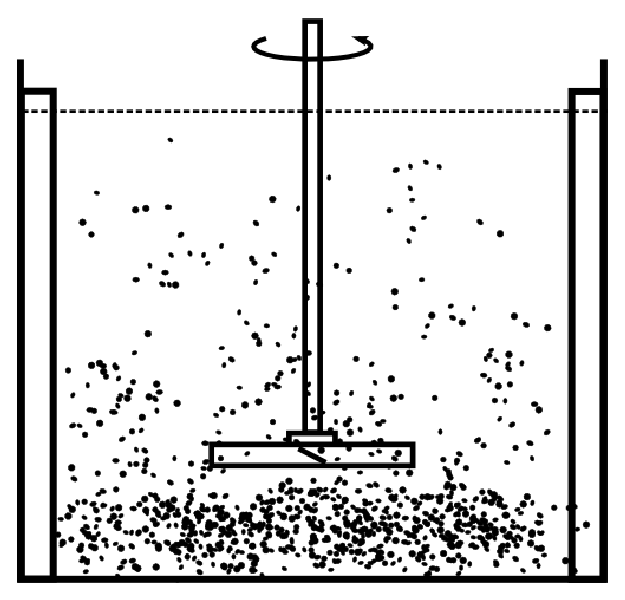
\includegraphics[scale=0.35]{images/typy_suspenzi-1.eps}}
  \qquad
  \subfloat[Úplná]{\label{fig:typ2}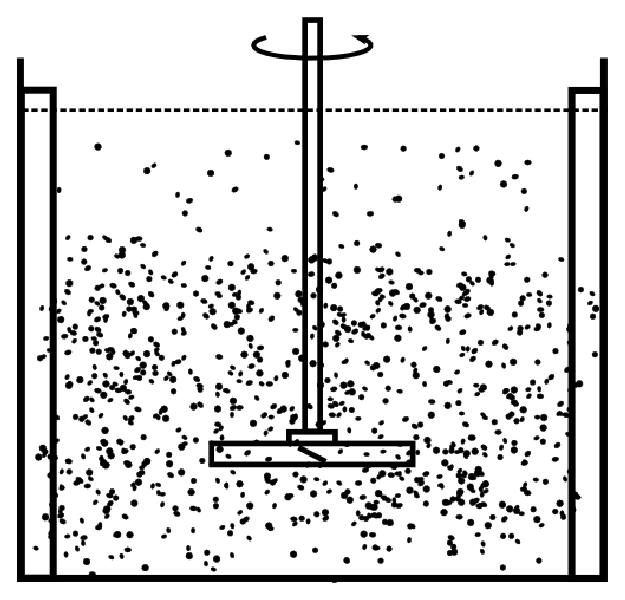
\includegraphics[scale=0.35]{images/typy_suspenzi-2.eps}}
  \qquad
  \subfloat[Homogenní]{\label{fig:typ3}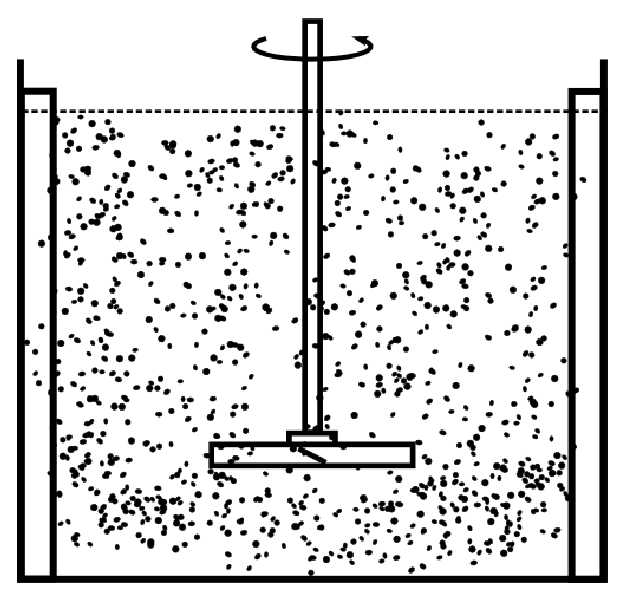
\includegraphics[scale=0.35]{images/typy_suspenzi-3.eps}}
  \caption{Stupně suspendace}
  \label{fig:typsus}
\end{figure}

Při částečné suspendaci lze vizuálně pozorovat pohyb částic pevné fáze pouze v~blízkosti dna nádoby. Toto shlukování má za následek zhoršení přestupu tepla a hmoty, což v~důsledku může snížit rychlost probíhajících chemických reakcí. Z~výše uvedeného vyplývá, že podmínky částečné suspendace jsou postačují pouze při míchaní vysoce rozpustných látek.

Stav úplné suspendace je charakterizován pohybem pevné fáze v~celé nádobě, přičemž žádná částice nezůstává na dně déle než jednu až dvě sekundy. Tato podmínka se někdy označuje jako Zwieteringovo kritérium podle autora, který jako první na základě experimentů navrhl vztah k~výpočtu kritické (minimální) frekvence otáčení míchadla potřebné k~dosažení stavu úplné suspendace. Při tomto stavu je maximální povrch částic vystaven kapalině, což má za následek intenzivní transport hmoty a tepla mezi jednotlivými fázemi.

Posledním stádiem je dosažení stavu homogenní suspendace, při němž částice pevné fáze dosahují prakticky rovnoměrného rozložení v~celém promíchávaném systému. Jakékoliv další zvýšení frekvence míchadla nebo jeho příkonu nemá již prakticky žádný vliv na distribuci pevné fáze. Dosažení stavu homogenní suspendace je často důležité u~procesů, které vyžadují rovnoměrné rozložení částic v~systému. Příkladem takovéhoto procesu může být krystalizace, kde nerovnoměrná koncentrace pevné fáze způsobuje tvorbu míst s~lokálním přesycením, jenž následně negativně ovlivňují kvalitu vzniklých krystalů. Nicméně ve většině případů je postačující dosažení stavu úplné suspendace, který vyžaduje menší množství vykonané práce.

\subsection{Kritická frekvence otáčení míchadla}
Jak již bylo zmíněno v~předcházející kapitole, kritická frekvence otáčení je minimální rychlost otáčení míchadla potřeba k~udržení částic pevné fáze ve vznosu. První kdo navrhl empirickou korelaci k~jejímu výpočtu byl \citet{zwi58}. Jím navržený vztah má tvar:

\begin{equation}
	N_{js} = \left[\frac{g(\rho_{s}-\rho_{l})}{\rho_{l}}\right]^{\num{0.45}}W^{\num{0.13}}d_{p}^{\num{0.2}}D^{\num{-0.85}}\nu^{\num{0.1}}S
	\label{eq:nkrit}
\end{equation} 

\noindent kde $g$ je gravitační zrychlení, $\rho_{s}$ hustota pevné fáze, $\rho_{l}$ hustota kapalné fáze, $W$ relativní hmotnostní zlomek pevné fáze, $d_{p}$ průměr částice pevné fáze, $\nu$ kinematická viskozita a $S$ je bezrozměrná Zwieteringova konstanta, která zohledňuje geometrii systému a míchadla (tab. \ref{tab:S}). Ze vztahu je dobře patrné, že rozdíl hustot jednotlivých fází nejvýznamněji ovlivňuje výslednou kritickou frekvenci otáčení míchadla. Později provedené studie \citep{nie68,bal78,chou97} obecně potvrdily platnost Zwieteringova vztahu. Nicméně \citet{chou97} experimentálně ukázal, že při koncentraci pevné fáze menší než \volproc{2} nebo větší než \volproc{15} se již tato korelace jeví jako nepříliš spolehlivá.

\begin{table}[h!]
\begin{center}
\caption{Zwieteringovy konstanty pro \SI{45}{\degree} PBT}
\label{tab:S}
\begin{tabular}{llr}
\toprule
Šířka lopatky & Světlá výška & Hodnota \\
\midrule

$D/\num{3.5}$ \\
& $T/4$ & \num{4.8} \\
& $T/6$ & \num{4.6} \\
& $T/8$ & \num{3.2} \\
$D/4$ \\
& $T/4$ & \num{4.4} \\
& $T/6$ & \num{4.1} \\
& $T/8$ & \num{3.7} \\

\bottomrule
\end{tabular}
\end{center}
\end{table}

\subsection{Kvalita suspenze (stupeň homogenizace)}
Další užitečnou charakteristikou systému kapalina-pevná fáze je takzvaná kvalita suspenze, což je směrodatná odchylka koncentrace pevné fáze.Často se však dává přednost vyjádření pomocí objemového zlomku pevné fáze. Pro konečný počet $n$ měření lze kvalitu suspenze definovat jako:

\begin{equation}
	\sigma = \sqrt{\frac{1}{n}\sum_{n}^{i=1}\left(\frac{c_{i}}{\bar{c}} - 1\right)^{2}}
	\label{eq:kvasus}
\end{equation}  

\noindent Díky své diskrétní povaze je tato veličina navíc dobře stanovitelná pomocí simulace technikou CFD.

\begin{table}[h!]
\begin{center}
\caption{Zwieteringovy konstanty pro \SI{45}{\degree} PBT}
\label{tab:jj}
\begin{tabular}{cc}
\toprule
Stupeň suspendace & Kvalita suspenze $(\sigma)$ \\
\midrule

Částečná & \num{4.8} \\
Úplná & \num{4.6} \\
Úplná & \num{4.6} \\

\bottomrule
\end{tabular}
\end{center}
\end{table}


\newpage 
\section{Počítačová dynamika tekutin (CFD)}




	\chapter{Literature review}
The suspension of solids has been investigated very extensively over the years. Pioneering was made by \citet{zwi58}, who provided an empirical dimensionless correlation for the  stirred speed at which solids are just suspended. For this velocity is characteristic that no particle remains stationary on the bottom of a tank for more than one or two seconds. Also other authors have experimentally studied the mechanism of suspension of solids in agitated vessels \citep{nie68,bal78,arm98}.   

In the last two decades many researchers have turned their attention to computational fluid dynamics in order to gain better understanding of the phenomena that govern the multiphase systems. Since then CFD has been increasingly employed as an essential tool to minutely analyze the entire flow field and the solid particle distribution. The early CFD simulations   

\section{Particle drag coefficient}


	\chapter{Experimentální část}
Experimentální studii suspendace v mechanicky míchané nádobě provedla Bc.\,Zuzana Pavlíková v rámci své bakalářské práce na Ústavu chemického inženýrství VŠCHT Praha v roce 2011.

\section{Popis experimentu}
Náplní experimentu bylo měření průběhu homogenizace kapaliny v přítomnosti pevné fáze a následném zjišťování doby homogenizace. K provedení experimentu byla využita válcová nádoba z plexiskla o vnitřním průměru $T=\SI{0.29}{\meter}$ s plochým dnem, jenž byla opatřena čtyřmi radiálními narážkami o šířce $b=T/10$. Výška plnění nádoby byla zvolena $H=T$. 

\begin{figure}[h!]
\begin{center}
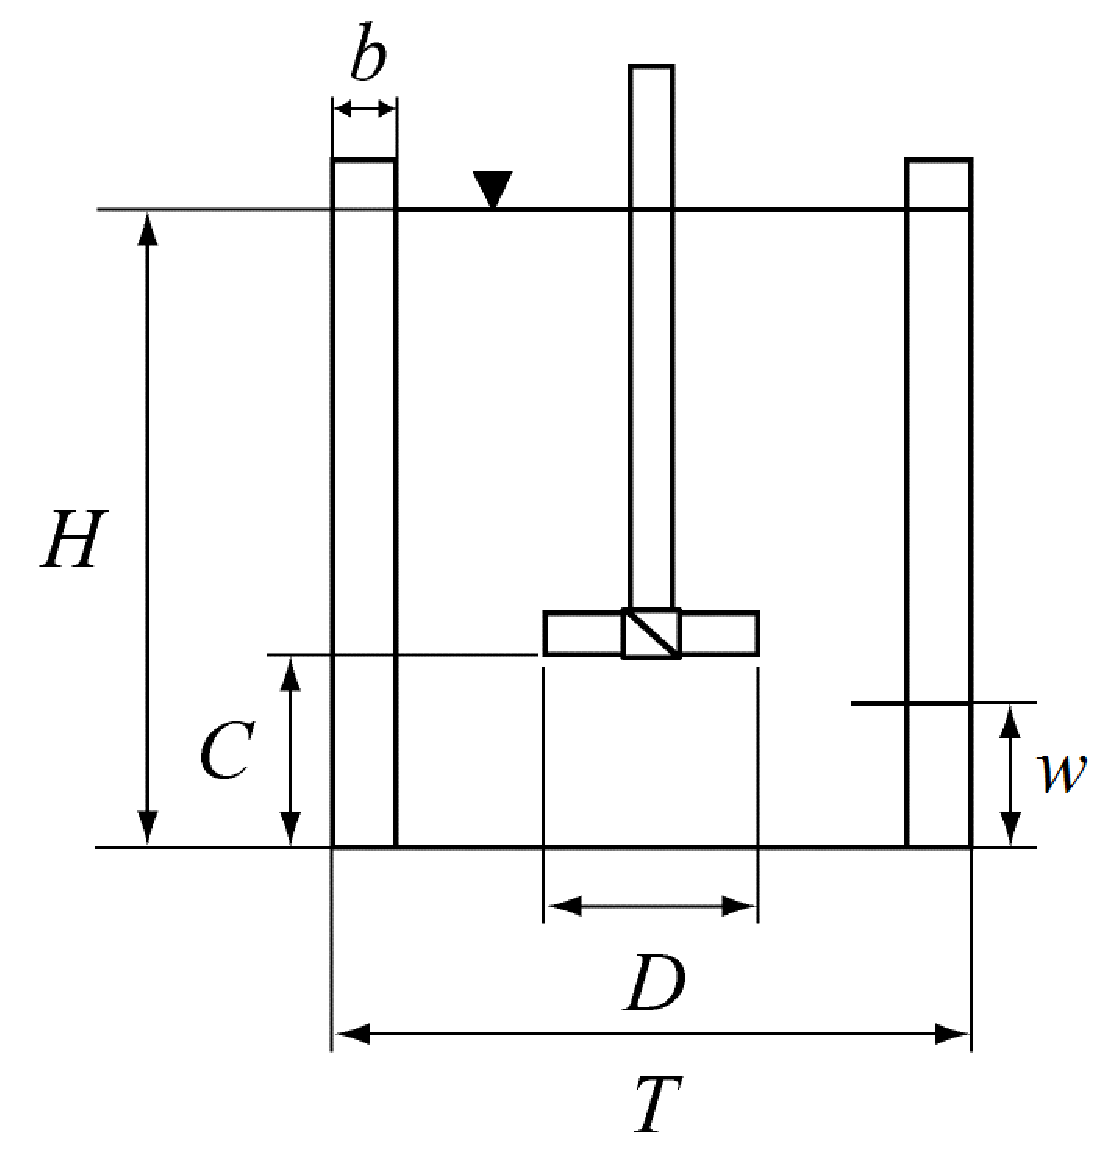
\includegraphics[scale=0.45]{images/mujedit.eps}
\caption{Geometrie experimentu}
\label{fig:nadoba}
\end{center}
\end{figure} 

Do nádoby $C=T/3$ ode dna bylo umístěno šestilopatkové míchadlo se šikmo skloněnými lopatkami (úhel zkosení \SI{45}{\degree}). Rychlost otáčení byla postupně volena  \SIlist[list-units = single]{3;4;5;6;7;8;9}{\per\second}. Celkový průměr míchadla činil $D=T/3$ a ostatní jeho rozměry jsou zobrazuje obr. XX.      

Jako vsádka byla použita voda a polyvinylpyrrolidon (PVP). Pevnou fázi tvořily červené kuličky z polyvinyl (PVC) o 

	\chapter{Výpočetní část}

\section{Tvorba geometrie a výpočetní sítě}

Prvním krokem před každou CFD simulací je tvorba geometrie systému a její následná diskretizace (tzv. vysíťování). Výpočetní doména byla vytvořena podle geometrie experimentu uvedené v~kapitole \ref{chap:exp} prostřednictvím programu ANSYS DesignModeler 12.1. Pro snížení výpočetní náročnosti byla simulována pouze část nádrže obsahující kapalinu bez přítomnosti vzduchu. Míchací nádoba byla rozdělena na část rotační, kterou tvořil válec, o výšce \SI{5.2}{\centi\meter} a průměru \SI{16.5}{\centi\meter}, obsahující míchadlo a část hřídele, přičemž spodní podstava tohoto válec byla umístěna ve vzdálenosti \SI{1.35}{\centi\meter} od spodní hrany míchadla. Zbývající část systému obsahující větší část hřídele, dno, stěny a narážky nádoby představovala stacionární oblast. Vytvořená geometrie systému je znázorněna na obr. \ref{fig:geo}, kde zelenou barvou je znázorněna rotační zóna kolem míchadla. 

\begin{figure}[h!]
\centering
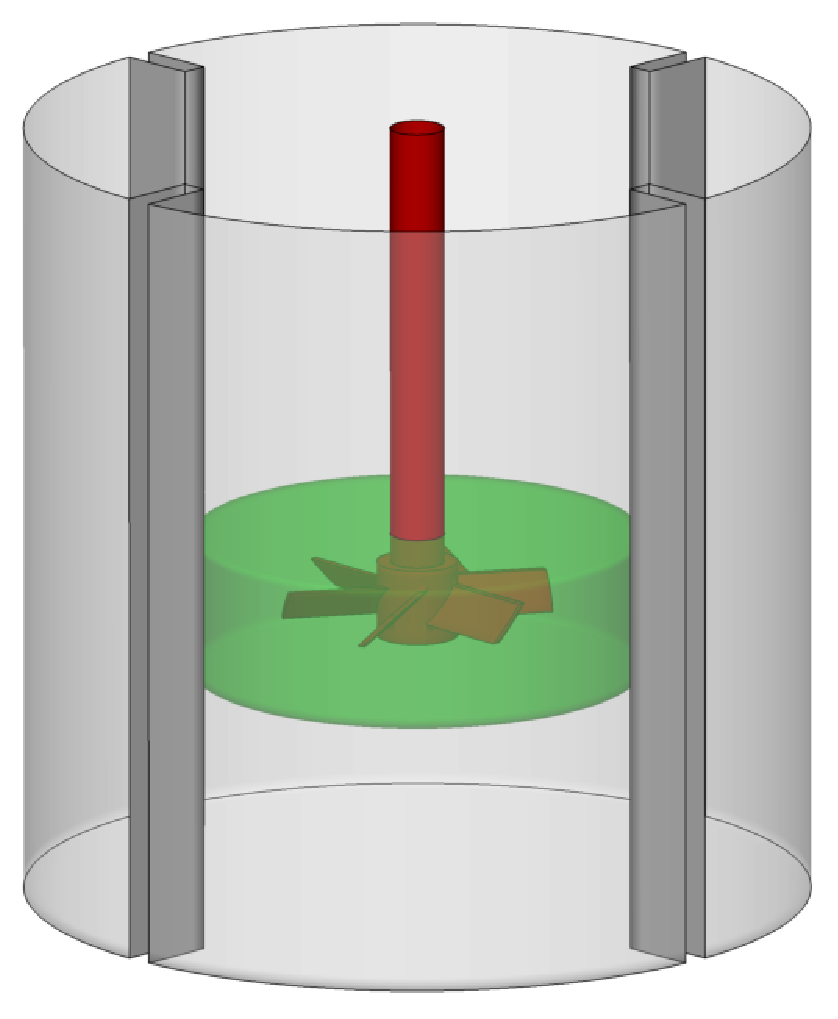
\includegraphics[scale=0.5]{images/geo.eps}
\caption{Geometrie systému}
\label{fig:geo}
\end{figure} 

Pro tvorbu výpočetní sítě byl využit program ANSYS Meshing 12.1 do kterého byla načtena geometrie nádoby vytvořená v předcházejícím kroku. Výslednou nestrukturovanou síť tvořilo \num{264398} buněk o průměrném objemu \SI{0.07}{\milli\litre}. Jednalo se převážně o šestistěnné buňky, přičemž pouze v oblasti pod míchadlem se vyskytovalo \num{132} třístěnných hranolů. Řez diskretizovanou doménou je zachycen na obr. \ref{fig:mesh} ze kterého si lze povšimnout, že ve spodní části nádoby je síť úmyslně zahuštěna. 
\begin{figure}[t]
\centering
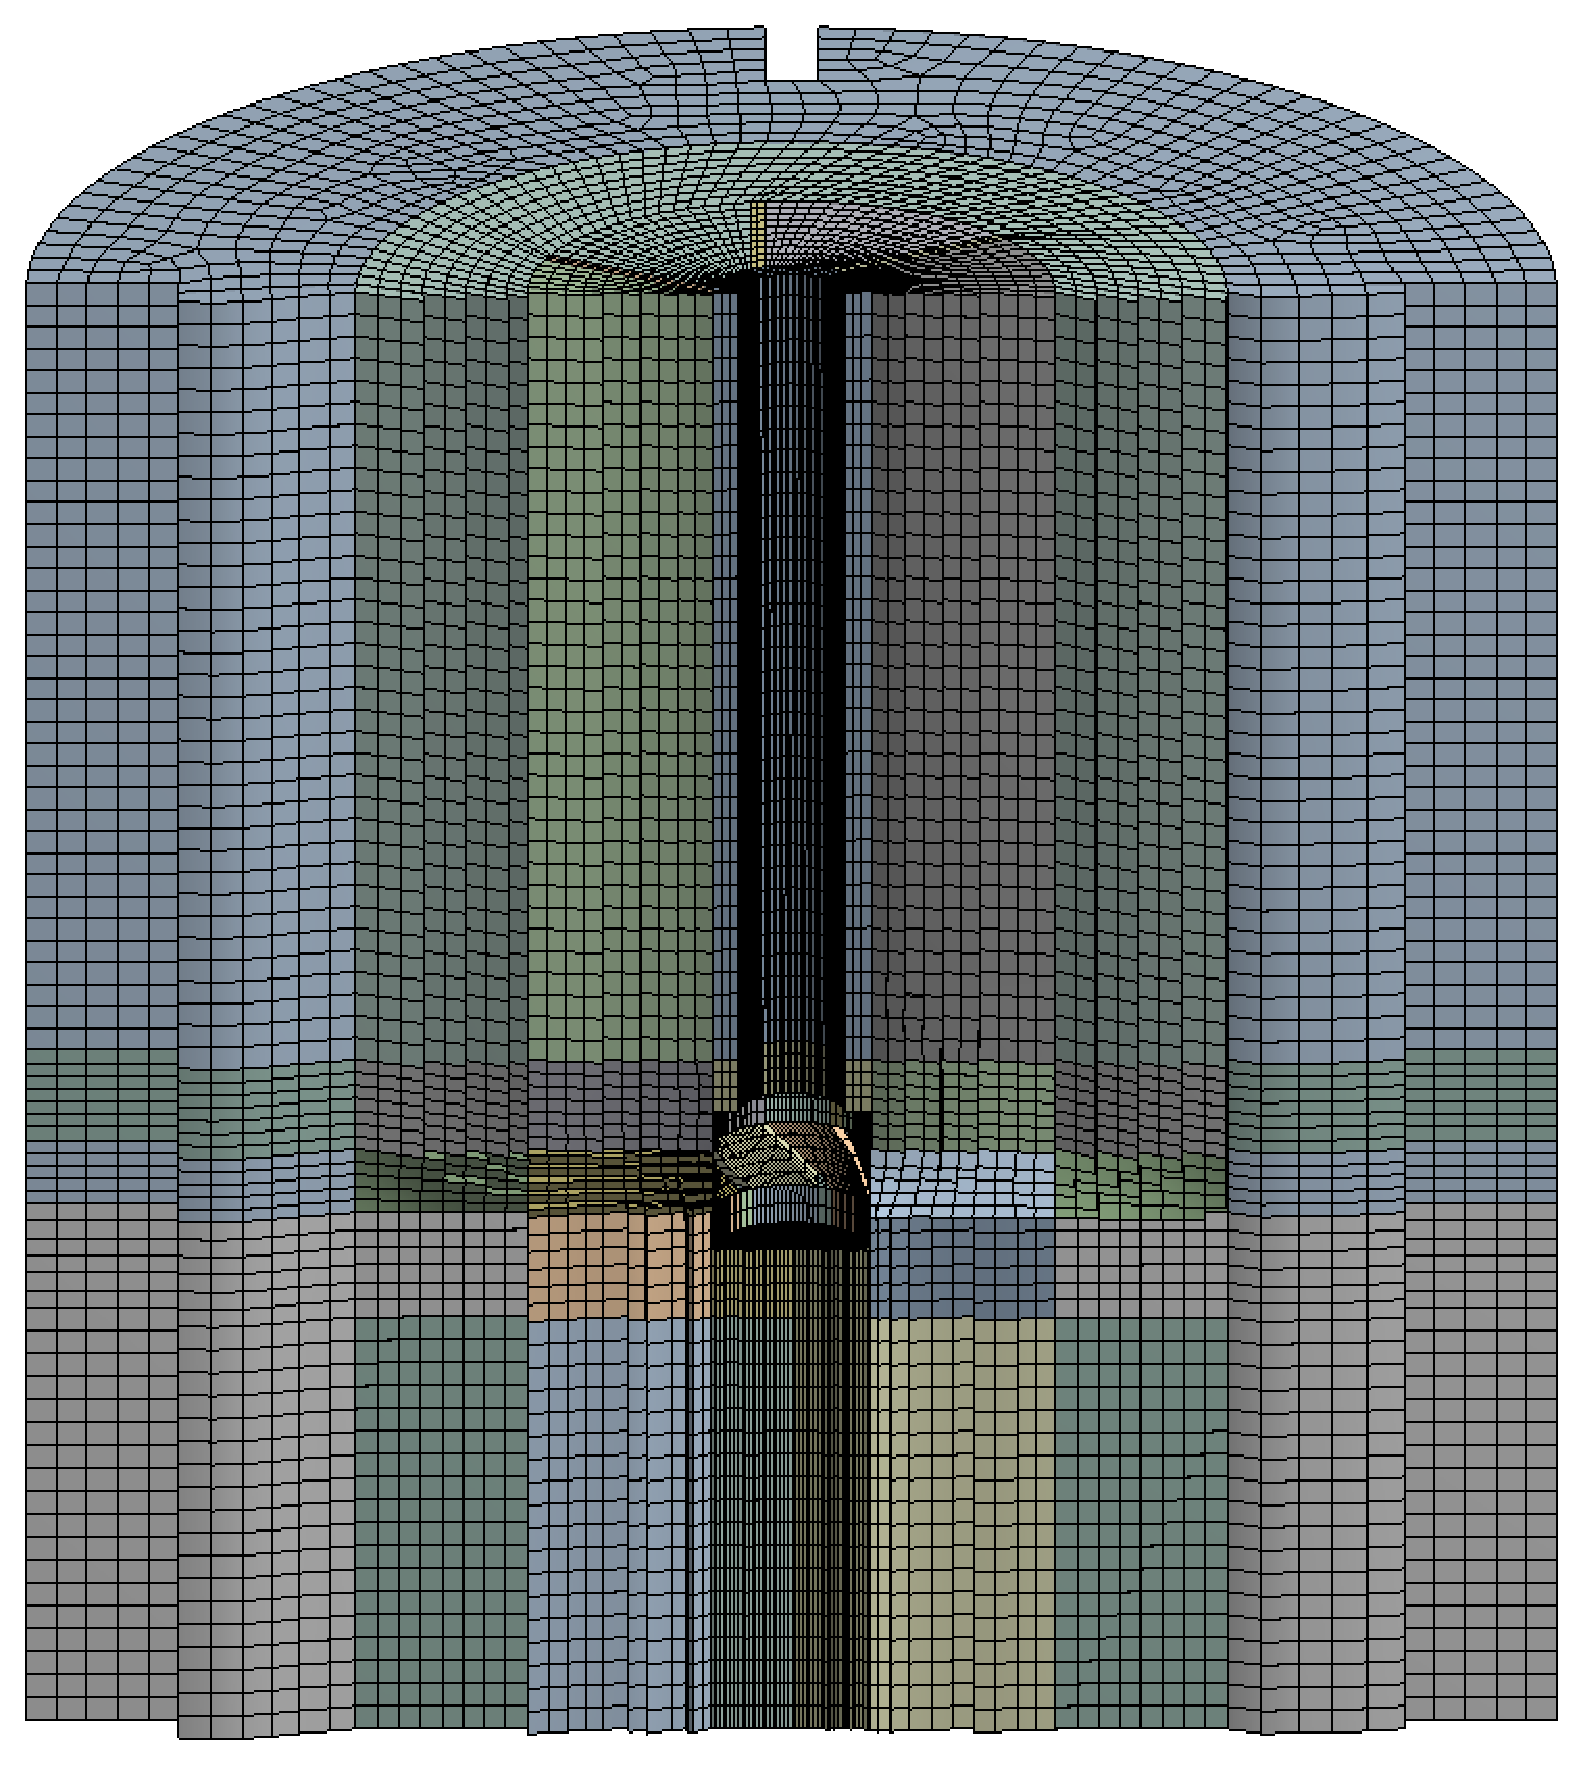
\includegraphics[scale=0.28]{images/mesh.eps}
\caption{Řez výpočetní sítí}
\label{fig:mesh}
\end{figure} 
Pro posouzení kvality vytvořené sítě existuje řada kritérií, avšak mezi nejpoužívanější patří tzv. šikmost (angl. skewness) definovaná jako:
\begin{equation}
      skewness = \mathsf{max}\kula{\frac{\beta_{max} - \beta_{e}}{180 - \beta_{e}}, \frac{\beta_{e} - \beta_{min}}{\beta_{e}}}
  	\label{eq:skw}
\end{equation} 
kde $\beta_{min}$, $\beta_{max}$ značí nejmenší resp. největší úhel v buňce a $\beta_{e}$ představuje úhel v pravidelném (ideálním) elementu. Šikmosti se obecně pohybuje v intervalu od \num{0} do \num{1}, přičemž nulová hodnota značí nejlepší kvalitu buňky, a naopak šikmost rovna jedné indikuje úplnou degeneraci elementu. Vybrané charakteristiky této veličiny pro vytvořenou výpočetní doménu jsou uvedeny v tab. \ref{tab:skw_tab}. Z uvedených hodnoty vyplývá, že vygenerovaná síť dosahuje výborné kvality.
\begin{table}[h!]
\centering
\caption{Charakteristiky šikmosti pro danou síť}
\label{tab:skw_tab}
\begin{tabular}{lr}
\toprule
\textbf{Charakteristika} & \textbf{Hodnota} \\
\midrule

Maximální šikmost & \num{0.666} \\
Průměrná šikmost & \num{0.164} \\
Směrodatná odchylka šikmosti & \num{0.123} \\

\bottomrule
\end{tabular}
\end{table}

\section{Uživatelem definované funkce}
Uživatelem definované funkce (UDF) jsou moduly načítané do softwaru \flu, jenž rozšiřují nebo upravují schopnosti řešiče. Například může se jednat o~definovaní vlastních počátečních a okrajových podmínek, změnu materiálových vlastností a modifikaci simulačních modelů. Pro tvorbu zdrojových souborů se využívá programovací jazyk C, které jsou následně zkompilovaný do dynamické knihovny.

Právě pomocí uživatelem definovaných funkcí byly implementovány modely pro koeficient odporu uvedené v~tab. \ref{tab:cds}. Navíc kromě korelací pro výpočet součinitele odporu byla do této knihovny naprogramována funkce pro výpočet kvality suspenze podle vztahu \ref{eq:kvasus}. Všechny vytvořené zdrojové kódy jsou uvedeny v kapitole \nameref{sec:priloha}.

\section{Vlastní CFD simulace}
Ke studiu suspendace pomocí CFD simulaci byl využit komerční software \flu{} 12.1.4 do kterého byla načtena vytvořená výpočetní síť. Následně byly nastaveny okrajové podmínky pro jednotlivé části řešené domény. Pro všechny fyzické části nádrže (dno, stěny, narážky, hřídel a míchadlo) byla vybrána okrajová podmínka typu stěna pro kterou platí, že rychlost na jejím povrchu je nulová. Z důvodu jednoduchosti byla pro hladinu kapaliny zvolena okrajová podmínka symetrie, jenž vyjadřuje nulovou hodnotu gradientu pro jednotlivé veličiny. Tato volba je obvyklá pro systémy kde je pozornost věnována dějům probíhající uvnitř nádoby, a nikoliv na mezifázovém rozhraní, což je právě případ suspendace. Pohyb rotační části domény byl v případě stacionární simulace modelován pomocí metody vícenásobných souřadnicových soustav (MRF) a pro nestacionární (dynamickou) simulaci byla použita technika klouzající sítě (SM). 

Proudění v nádobě bylo považováno za izotermní, nestlačitelné a s plně turbulentní. Pro popis turbulence byl standardní \keps{} turbulentní s disperzní modifikací pro vícefázový systém.



Množství pevné fáze v~míchací nádobě bylo zvoleno 5\,obj.\,\% pro všechny provedené výpočty. Jako vsádka byla zvolena kapalina PVP\,5, jejiž vlastnosti jsou uvedeny v~tab. \ref{tab:fyzvlast}. Pohyb míchadla byl simulován pomocí metody rotující sítě (sliding mesh) a jeho rychlost otáčení byla zvolena \SI{7}{\per\second}. Model Eulerian-Eulerian byl vybrán k~simulaci vícefázového proudění a pro popis turbulentního proudění byl využit standardní $k\mbox{-}\epsilon$ model s~disperzní modifikací. Časový krok nestacionární simulace byl zvolen \num{0.001} sekundy. Postupně byly využity všechny korelace pro koeficient odporu uvedeny v~tab. \ref{tab:cds} spolu s~klasickým Schillerovým-Naumannovým vztahem. 

Simulace probíhala na počítači HP Z600 osazený dvěma procesory Intel Xeon X5570 a pamětí 24 GB s~operačním systémem CentOS 5.3 x86-64. Doba výpočtu jedné reálné vteřiny trvala přibližně 4 hodiny.



  \chapter{Výsledky a diskuze}
Následující kapitola shrnuje výsledky provedených CFD simulací suspendace v mechanicky míchané nádobě. Navíc kde to situace umožňovala byly získaná data porovnány s dostupným experimentálním měřením.

\section{Rychlostní pole v nádobě}
Pro porovnání vlivu zvoleného turbulentního modelu na výsledné rychlostní pole bylo provedeno několik stacionárních simulací míchaní vodné vsádky. 

Na obr. \ref{fig:velfield} jsou znázorněno vektorové pole rychlosti kapaliny v~řezu nádobou pro jednotlivé turbulentní modely a frekvenci otáčení míchadla \SI{7}{\per\second}. Ze všech obrázků je dobře patrný vznik primární cirkulační smyčky která je charakteristická pro axiální míchadla. Navíc si lze také povšimnout tvorby sekundárních cirkulačních smyček v~prostoru pod míchadlem. Tento jev byl například experimentálně pozorován autory \citet{hos10} při zvolené světlé výšce míchadla od $C=T/2$ do $C=T/6$. Důležitý je také fakt, že i při srovnání s výpočetně náročnějším Reynoldsovým napěťovým modelem (obr. \ref{fig:RMS}) se jednotlivá rychlostní pole od sebe významně neliší.

\begin{figure}[h!]
 \centering

  \subfloat[Standardní \keps{}]{\label{fig:std}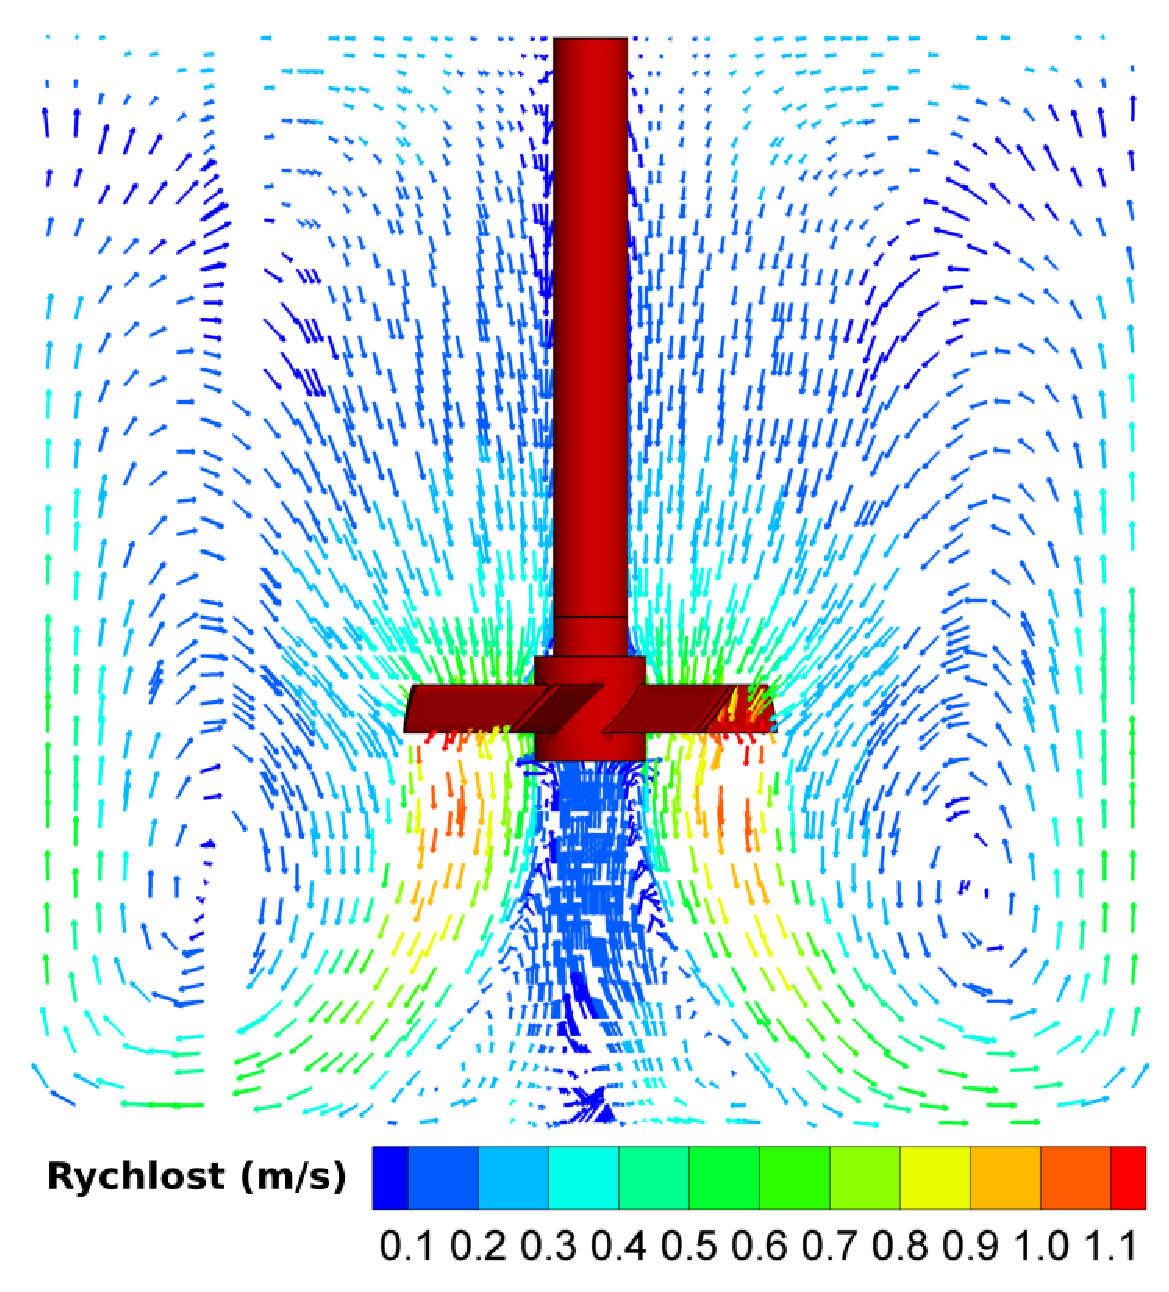
\includegraphics[scale=0.38]{Results/Velocity/keps-std.eps}}  
  \qquad 
  \subfloat[RNG \keps{}]{\label{fig:rng}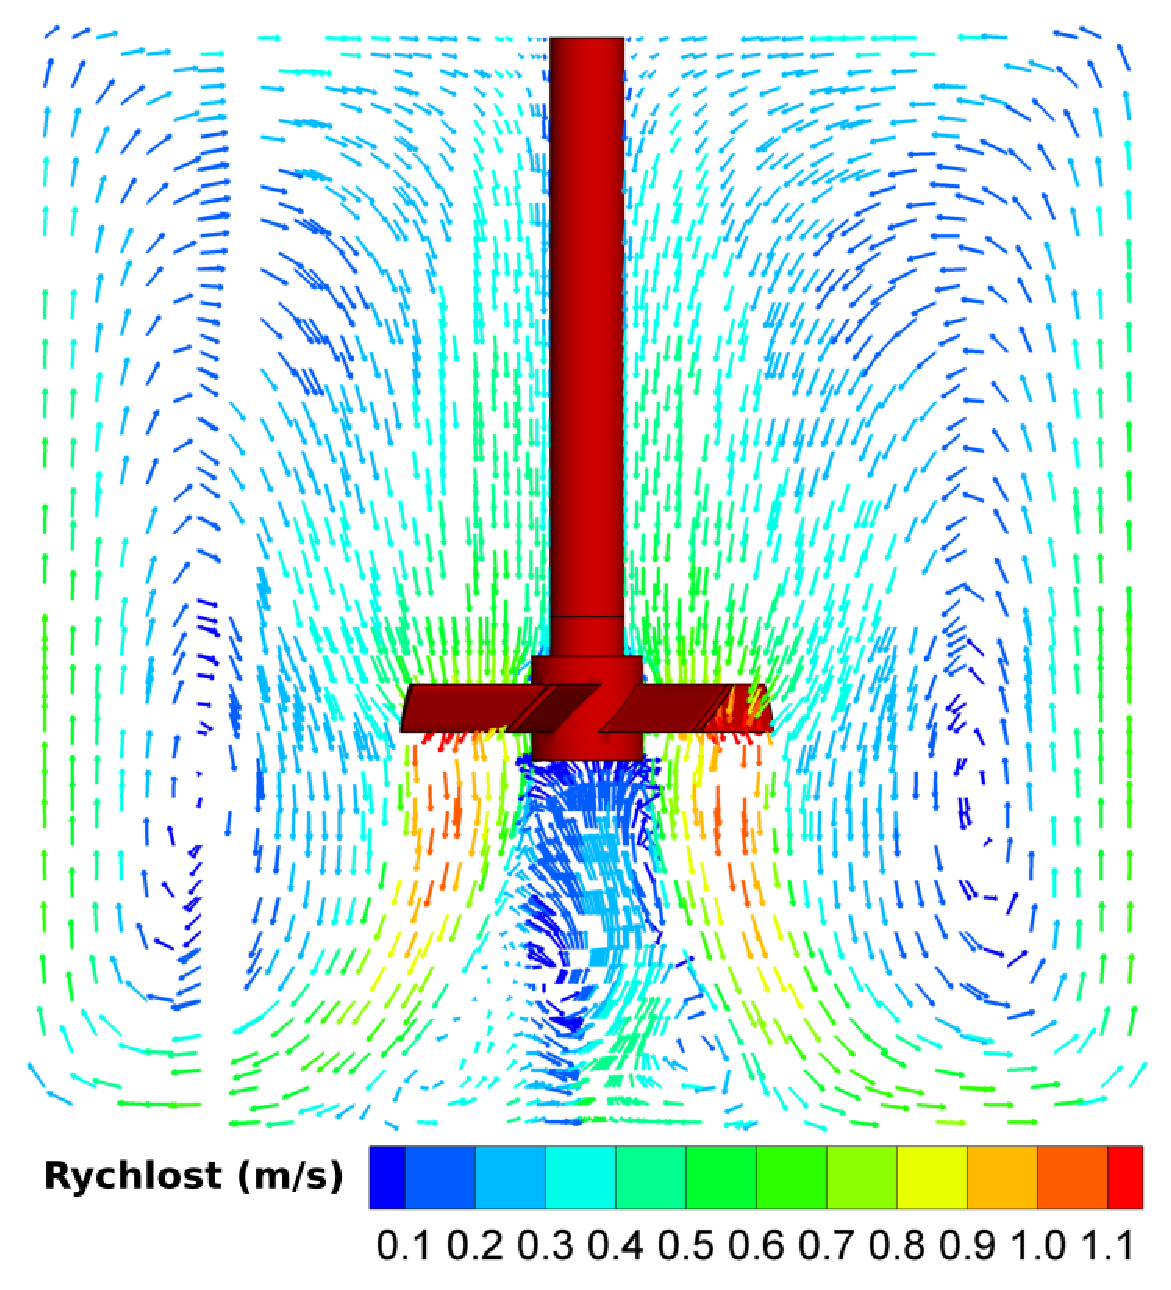
\includegraphics[scale=0.38]{Results/Velocity/keps-RNG.eps}}
\end{figure}
\newpage
\begin{figure}[t!]
  \addtocounter{subfigure}{2}
 \centering
  \subfloat[Realisable \keps{} ]{\label{fig:real}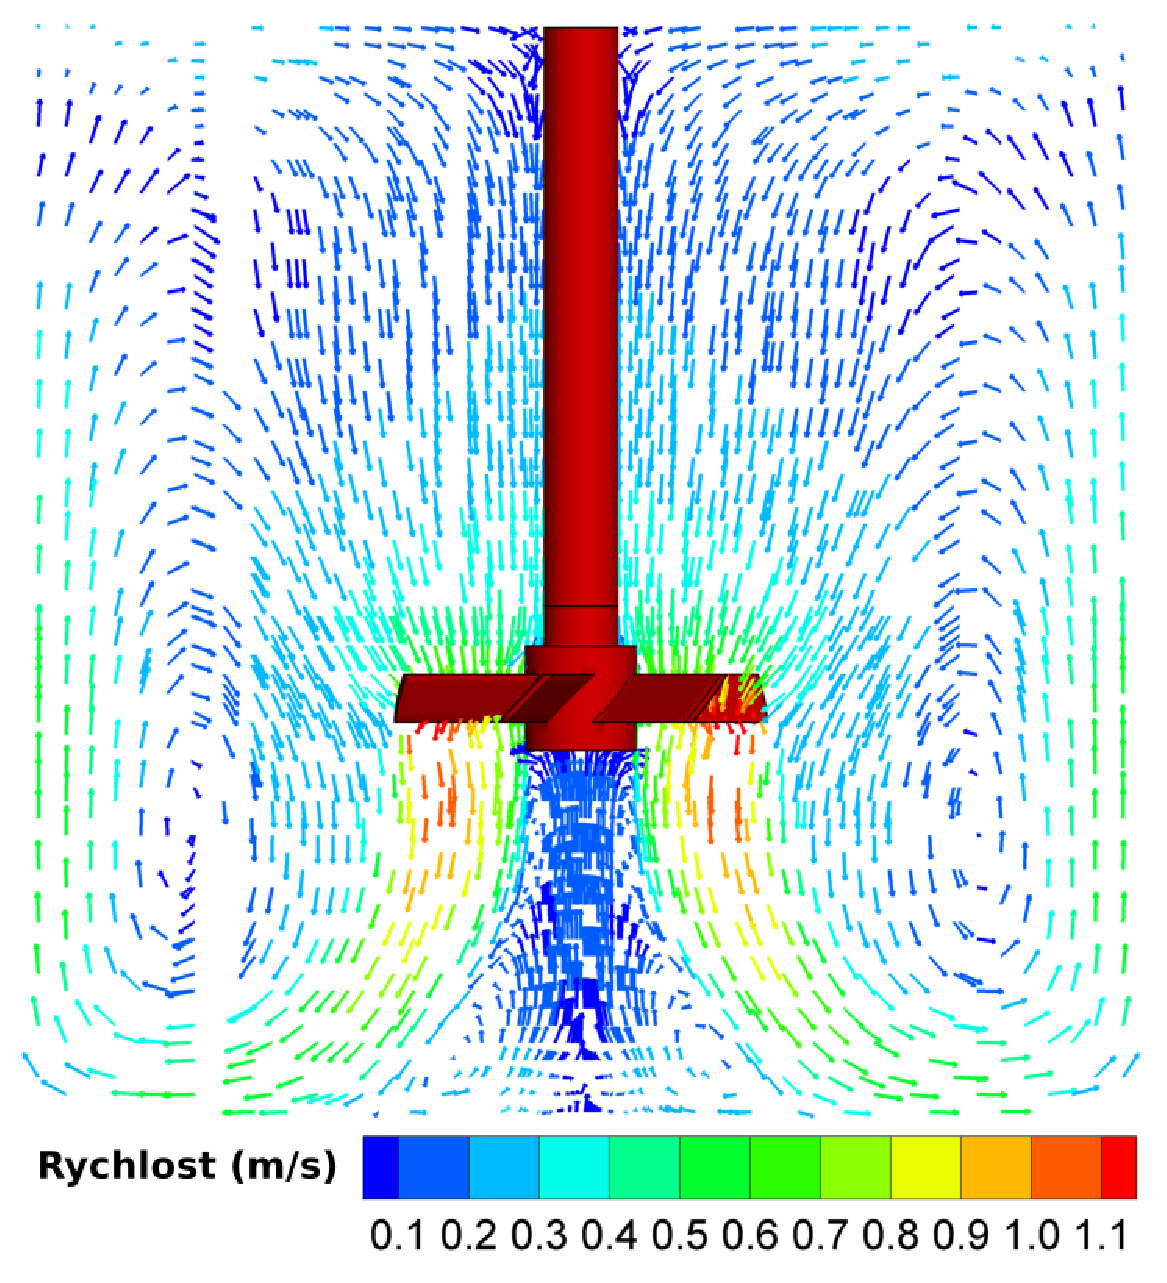
\includegraphics[scale=0.38]{Results/Velocity/keps-real.eps}}
  \qquad
  \subfloat[Standardní RMS]{\label{fig:RMS}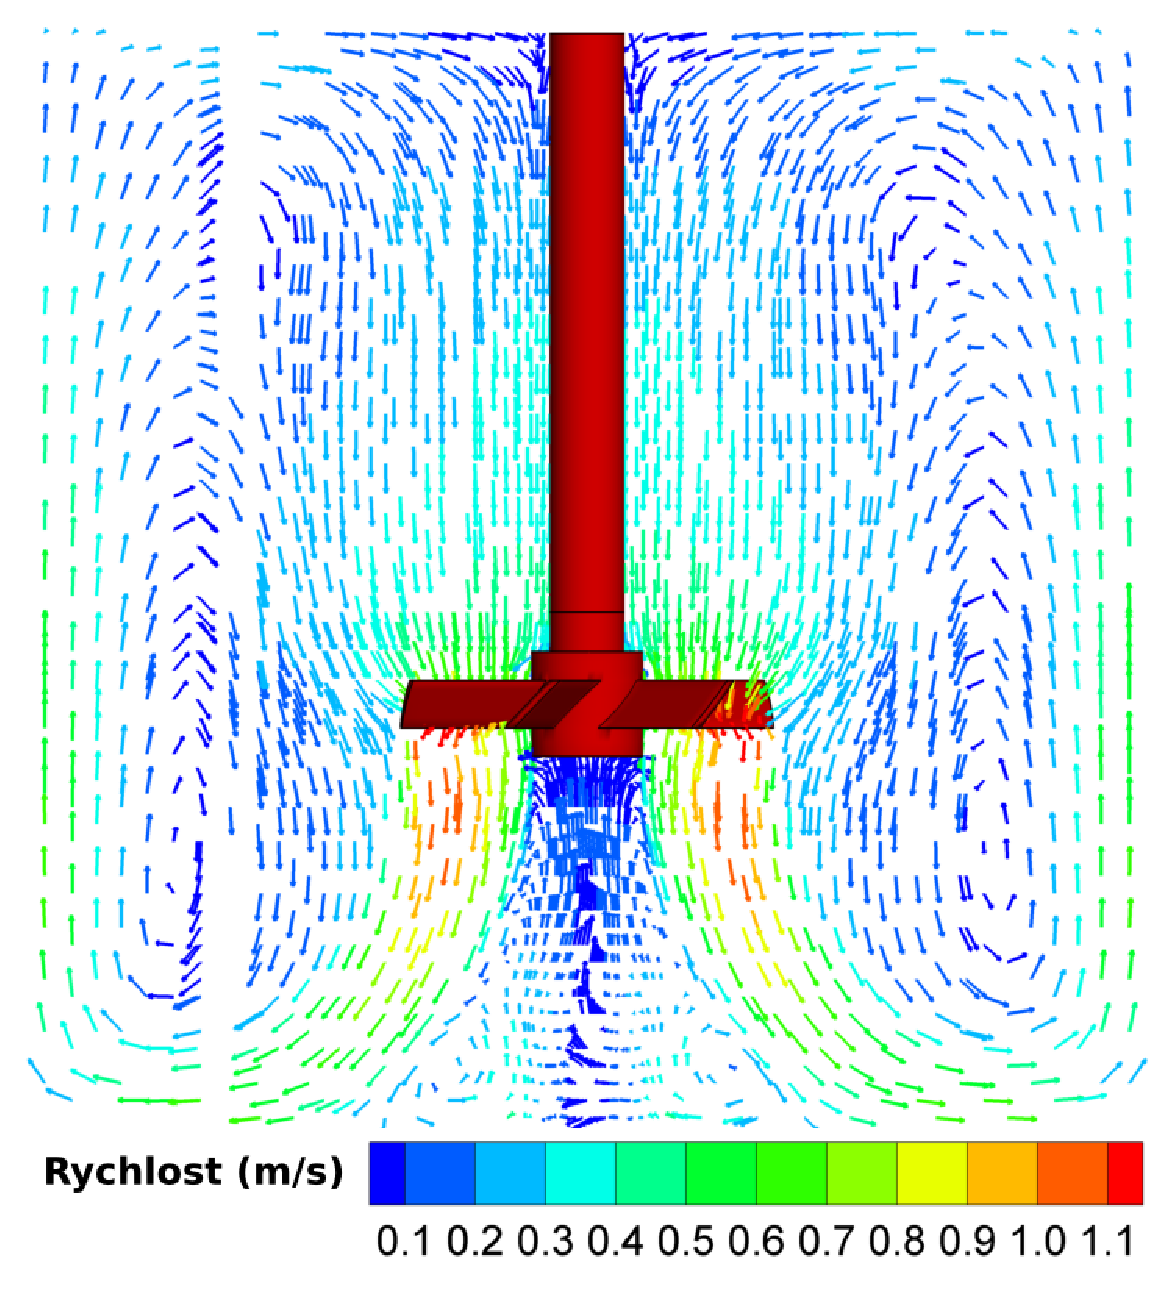
\includegraphics[scale=0.38]{Results/Velocity/RMS.eps}}
  \caption{Vektorové pole rychlosti pro různé turbulentní modely}
  \label{fig:velfield}
\end{figure}

Graf \ref{grf:velfield} zachycuje závislost mezi celkovou rychlostí pohybu kapaliny a vzdáleností ode dna nádoby ($y$) pro jednotlivé turbulentní modely. Konkretní hodnoty pro tento byly získány ve vzdálenosti \SI{0.5}{\centi\meter} podél jedné z narážek nádoby. Z grafu je dobře patrné, že u dna nádrže dochází nárůstu rychlosti tekutiny vlivem působení primární cirkulační smyčky.

\begin{grf}[h!]
 \centering
  \includegraphics[scale=0.45]{Results/Velocity/velField.eps}
  \caption{Průběh velikosti rychlosti tekutiny v nádobě}
  \label{grf:velfield}
\end{grf}

\section{Srovnání modelů pro koeficient odporu}
Jednotlivé modely pro koeficient odporu uvedené v podkapitole \ref{kap:cd} byly porovnány během nestacionární simulace systému obsahující jako vsádku \volproc{5} kuliček z PVC a kapalinu \pvpP. Rychlost otáčení míchadla byla v tomto případě opět nastavena na \SI{7}{\per\second}.

Obr. \ref{fig:cd2} zobrazuje kontury objemového zlomku pevné fáze v~řezu míchací nádobou pro vybrané korelace koeficientu odporu. Tyto údaje byly získány v~času simulace \SI{2}{\second}. 
\begin{figure}[h!]
 \centering

  \subfloat[Schiller-Naumann]{\label{fig:neu2}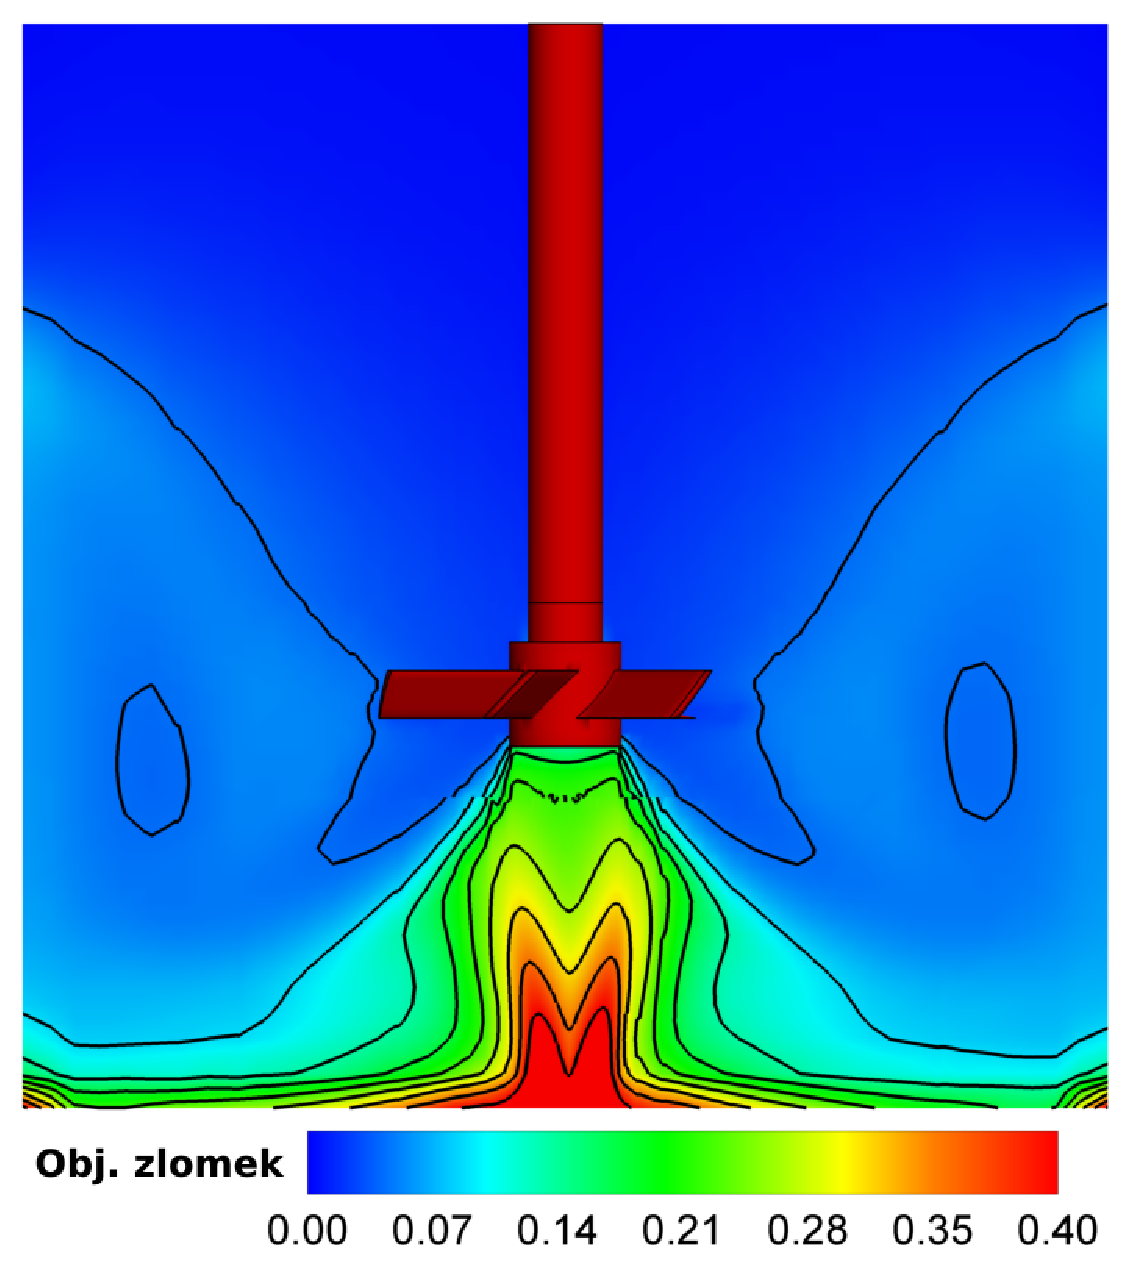
\includegraphics[scale=0.38]{Results/CDComp/neu-2s.eps}}  
  \qquad             
  \subfloat[{Brucato}]{\label{fig:bru2}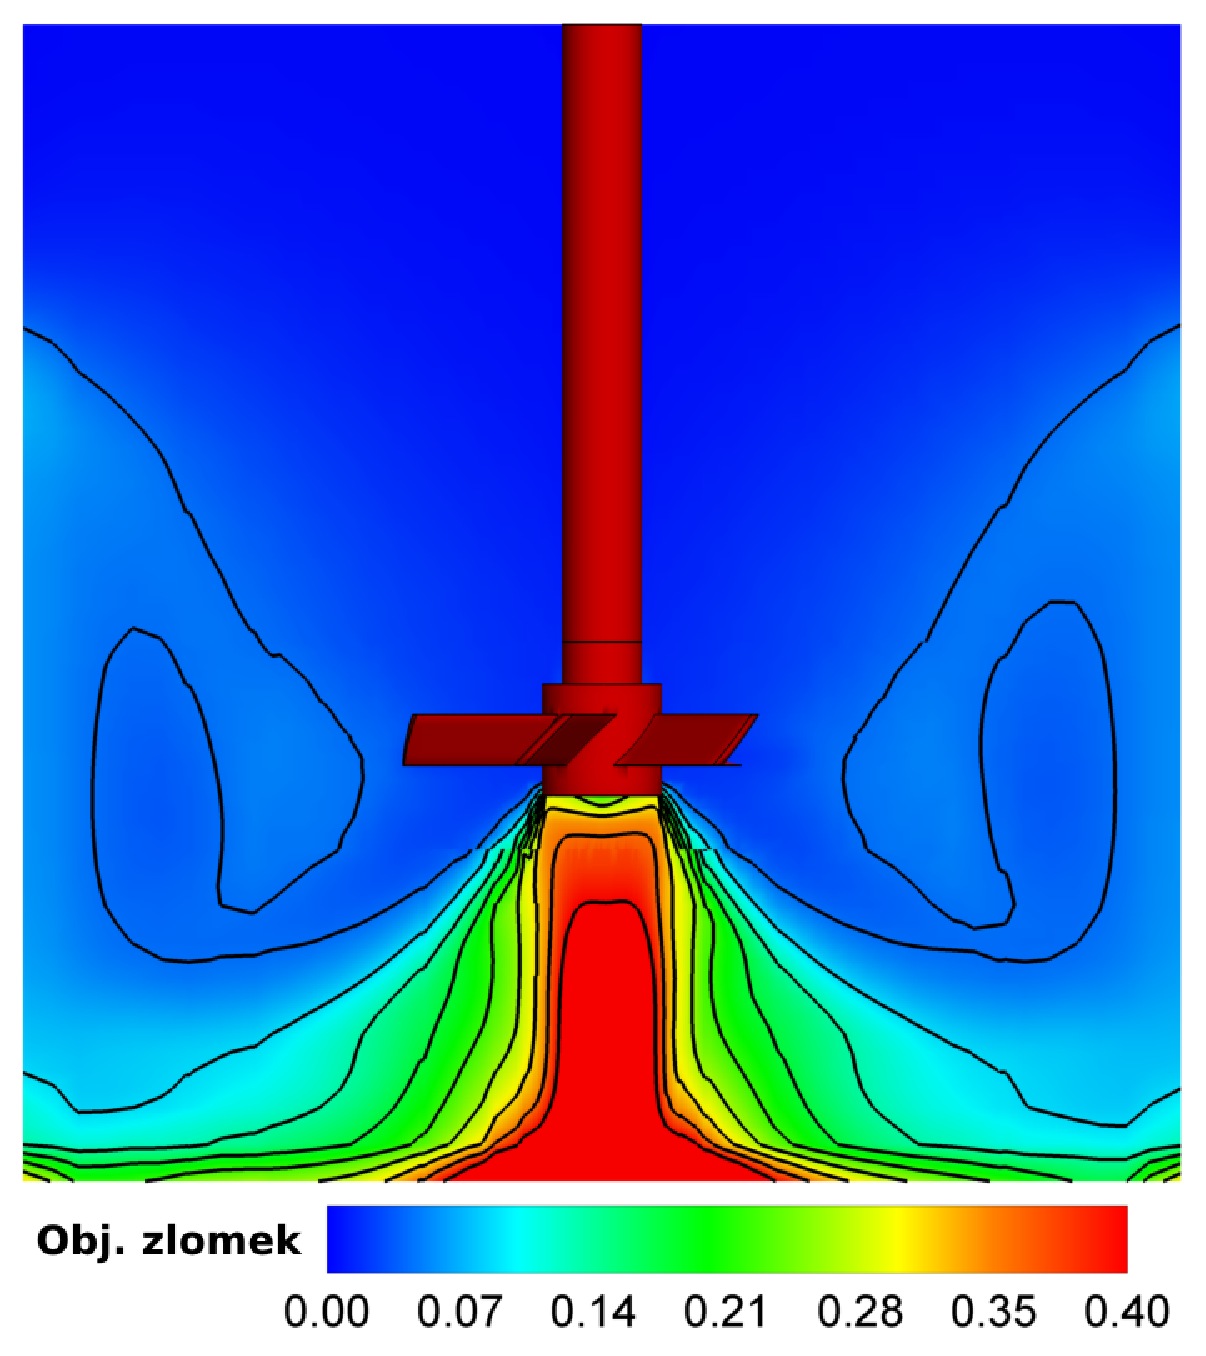
\includegraphics[scale=0.357]{Results/CDComp/bru-2s.eps}}
%\end{figure}
%\newpage
%\begin{figure}[t!]
	%\centering{}
  %\addtocounter{subfigure}{2}
  \\
  \subfloat[{Pinelli}]{\label{fig:pin2}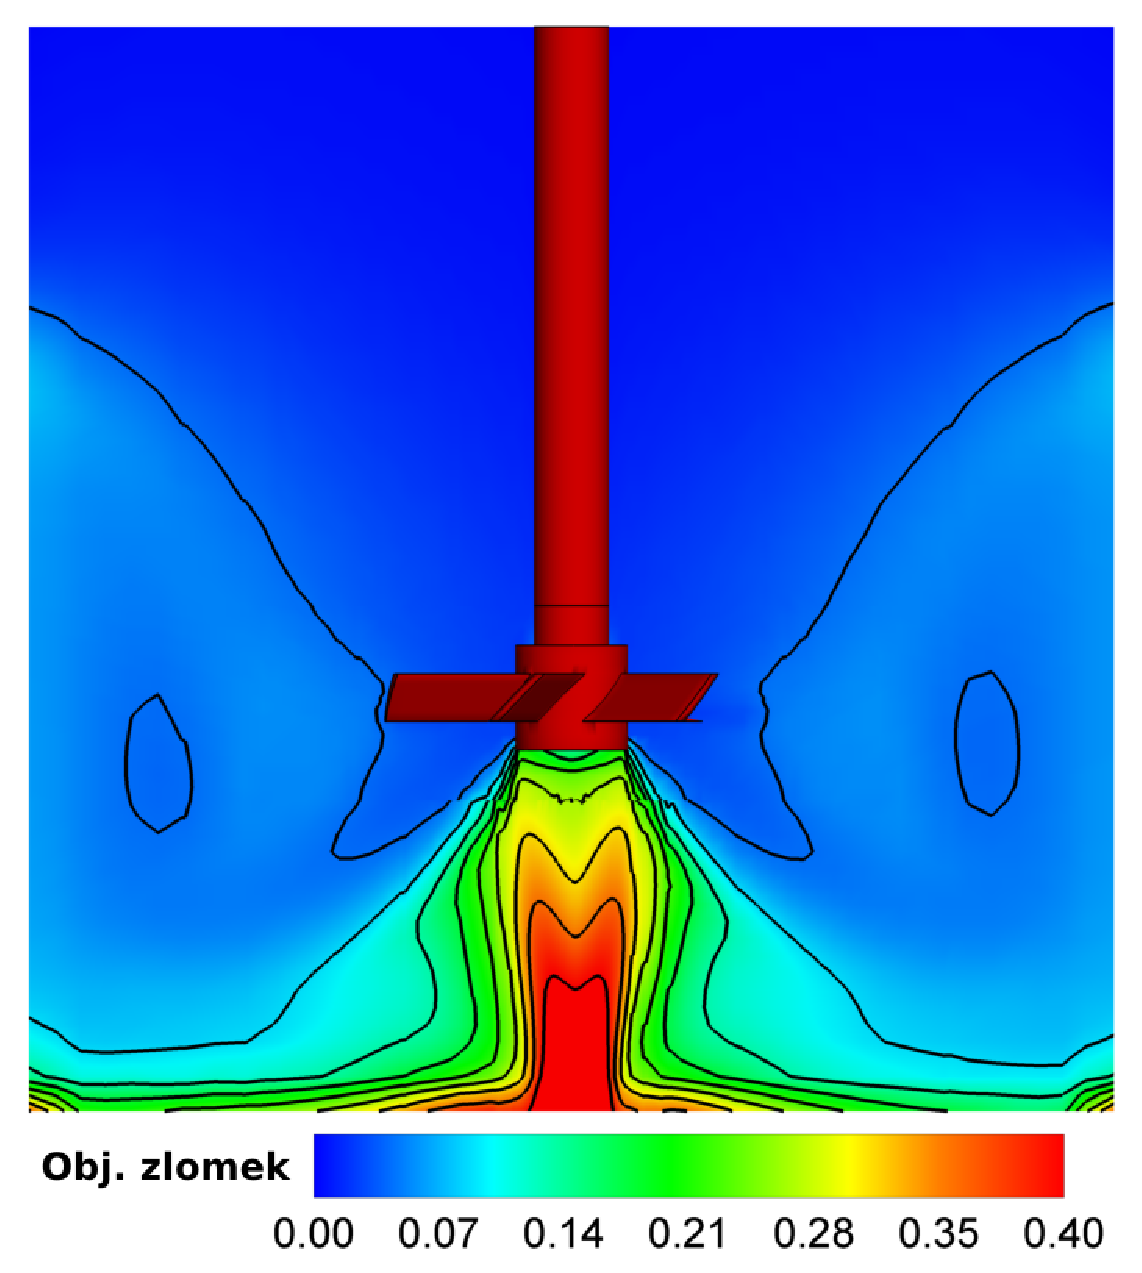
\includegraphics[scale=0.38]{Results/CDComp/pin-2s.eps}}
  \qquad
  \subfloat[{Khopkar}]{\label{fig:kho2}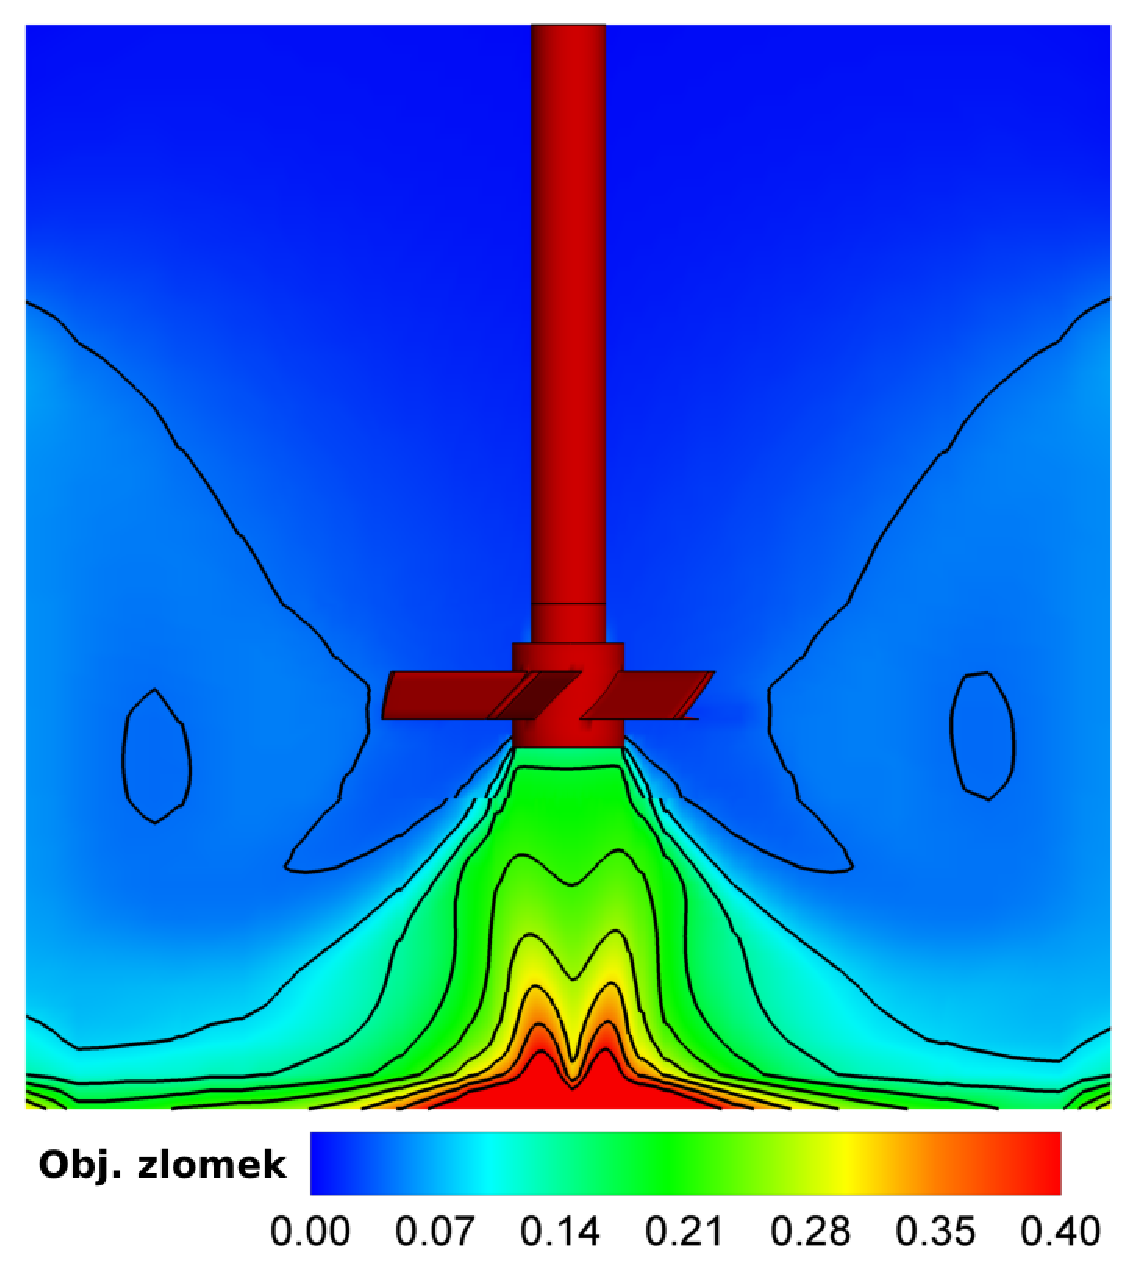
\includegraphics[scale=0.38]{Results/CDComp/kho-2s.eps}}
  \caption{Objemový zlomek pevné fáze v~čase \SI{2}{\second}}
  \label{fig:cd2}
\end{figure}
\newpage
\noindent Z~obrázků je dobře patrné, že přímo pod míchadlem je největší koncentrace pevné fáze vlivem sekundárních cirkulačních smyček, což se podařilo pozorovat i během experimentálního měření.

Série obrázků \ref{fig:cd7} zachycuje objemový zlomek pevné fáze v~řezu nádobou, avšak v čase simulace \SI{7}{\second}. Částice z PVC jsou již značně rozptýleny, ale stále se pod míchadlem nachází oblasti s jejich zvýšenou koncentrací. Nicméně v celé nádobě jsou rozdíly v distribuci pevné fáze mezi jednotlivými modely pro koeficient odporu poměrně zanedbatelné.

\begin{figure}[h!]
 \centering
  \subfloat[Schiller-Naumann]{\label{fig:neu7}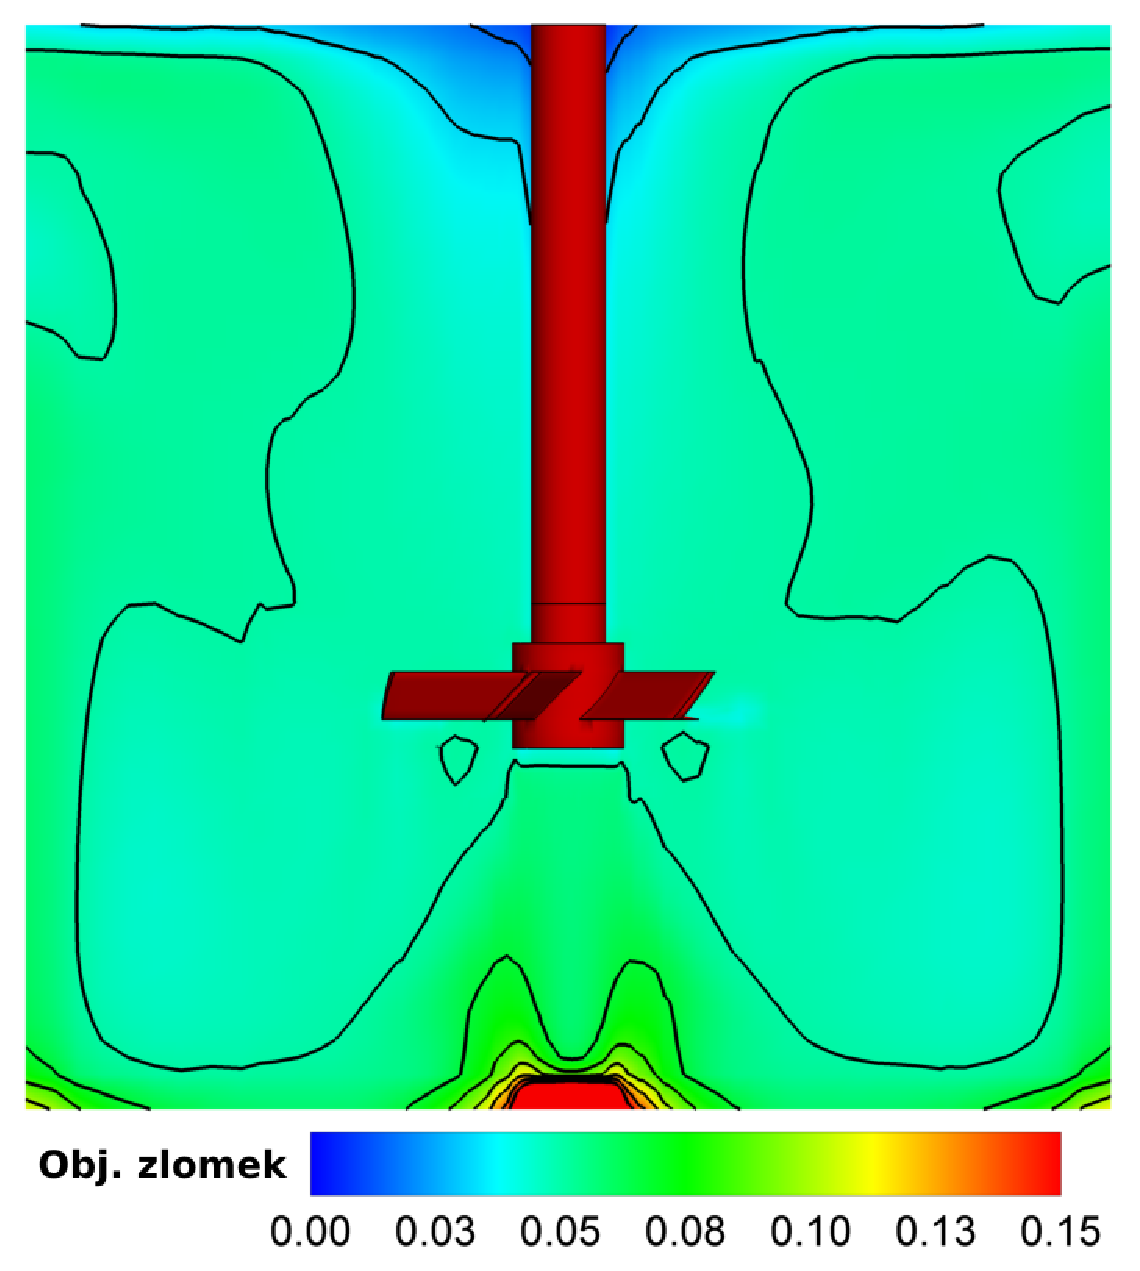
\includegraphics[scale=0.38]{Results/CDComp/neu-7s.eps}}  
  \qquad             
  \subfloat[{Brucato}]{\label{fig:bru7}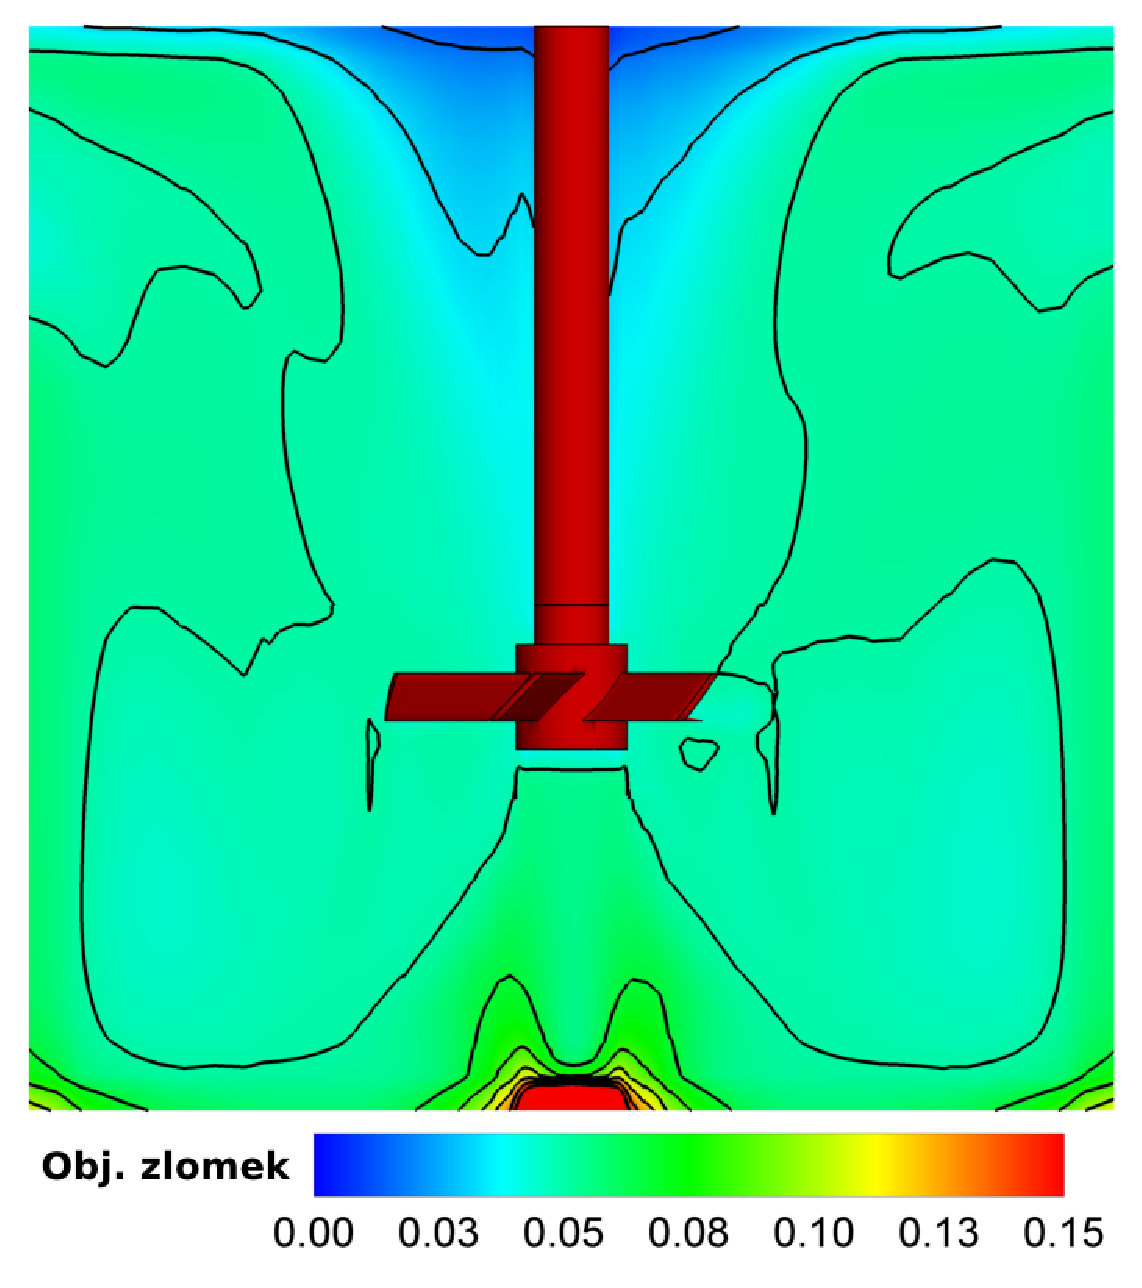
\includegraphics[scale=0.38]{Results/CDComp/bru-7s.eps}}
%\end{figure}
%\newpage
%\begin{figure}[t!]
	 %\centering{}
	 \\
  \subfloat[{Pinelli}]{\label{fig:pin7}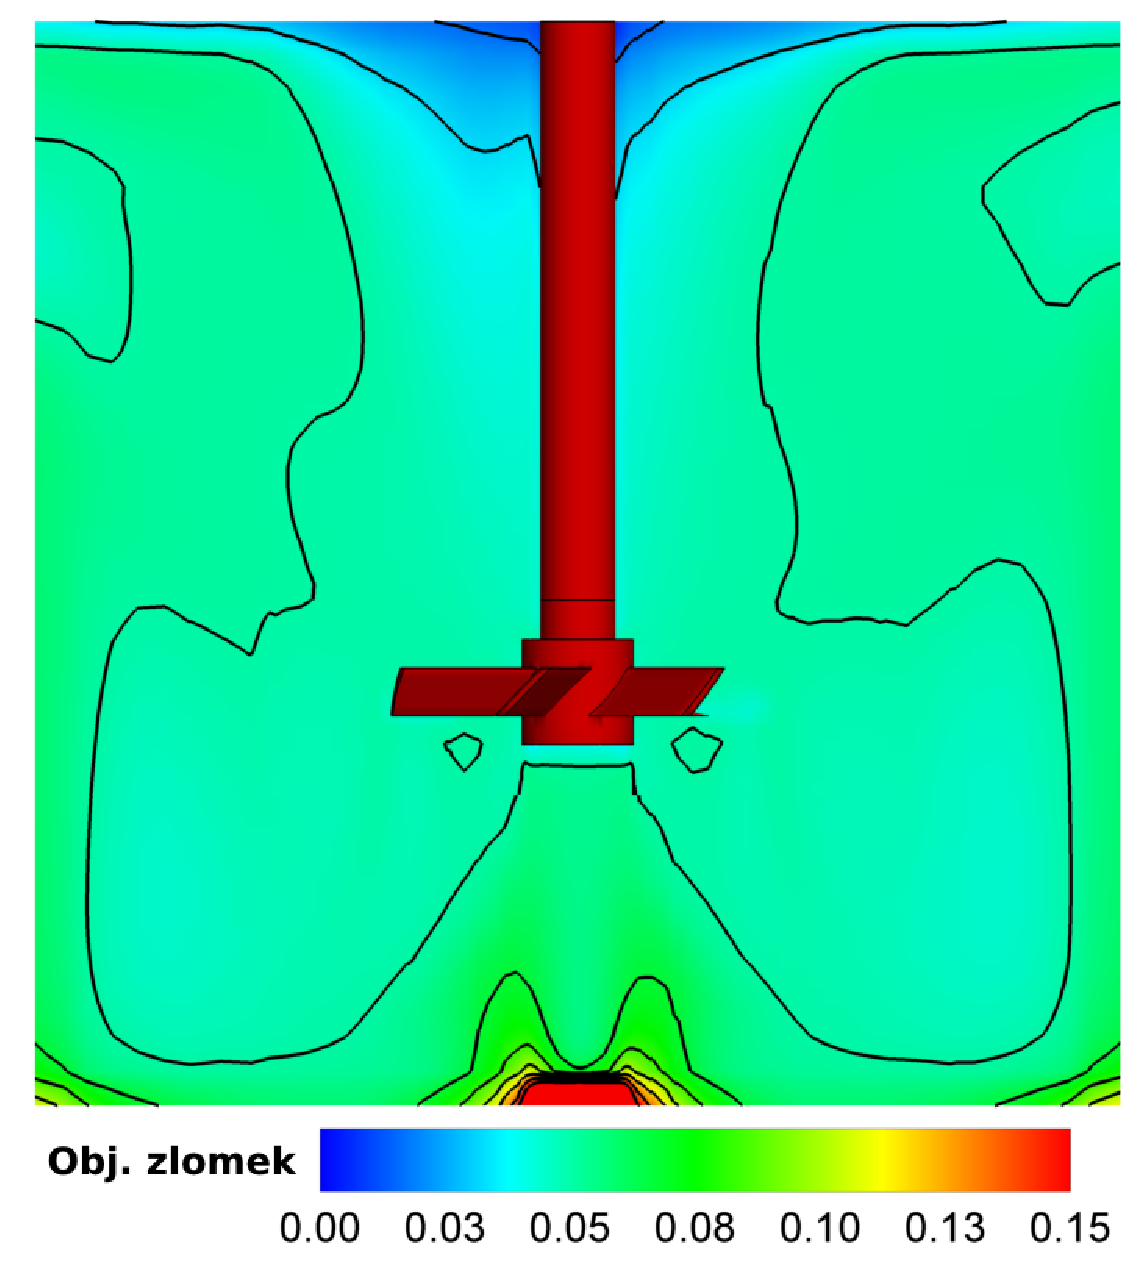
\includegraphics[scale=0.38]{Results/CDComp/pin-7s.eps}}
  \qquad
  \subfloat[{Khopkar}]{\label{fig:kho7}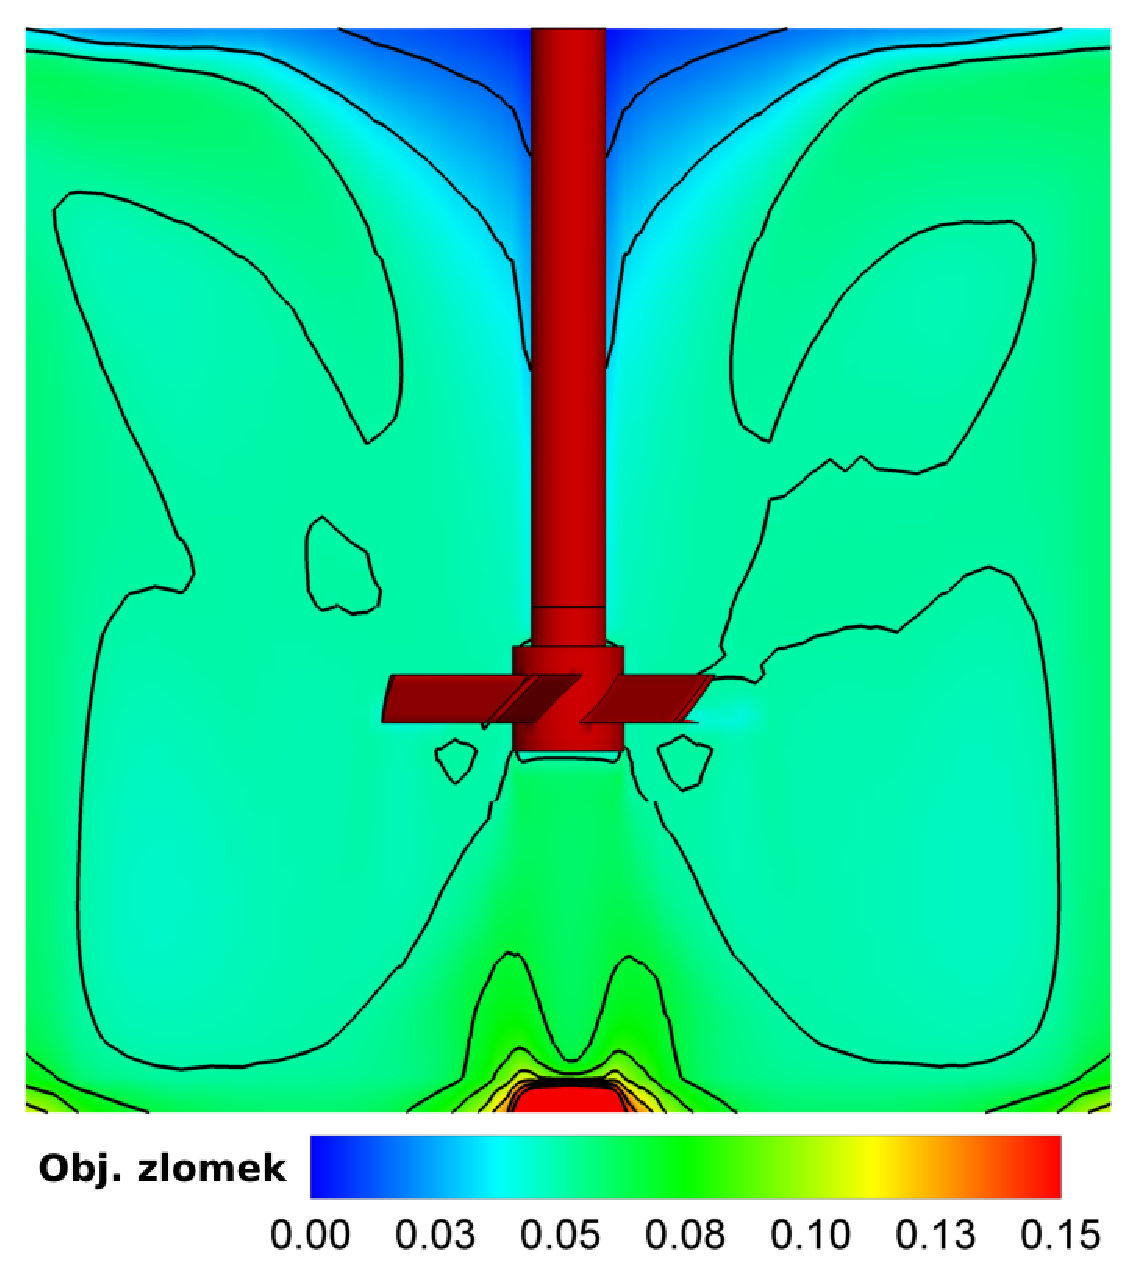
\includegraphics[scale=0.38]{Results/CDComp/kho-7s.eps}}
  \caption{Objemový zlomek pevné fáze v~čase \SI{7}{\second}}
  \label{fig:cd7}
\end{figure}
\newpage
\vspace{-5mm}
Dále jsou zde uvedeny grafické závislosti objemového zlomku pevné fáze na vzdálenosti ode dna nádoby. Z grafu \ref{fig:vol-2} lze vidět, že s~rostoucí vzdáleností se koncentrace pevné fáze postupně snižuje. Avšak grafická závislosti nemá monotonní průběh, přičemž dochází k~tvorbě esovitého koncentračního profilu. Model koeficientu odporu navržený Brucatem předpovídá nižší koncentraci pevné fáze ve vyšší vzdálenosti ode dna než zbylé tři modely. V~čase \SI{7}{\second} kuličky z~PVC již dosáhly značného vznosu a rozdíly mezi jednotlivými korelace pro koeficient odporu se začínaly vytrácet (viz. graf \ref{fig:vol-7}).
\begin{grf}[h!]
 \centering
  \subfloat[v~čase \SI{2}{\second}]{\label{fig:vol-2}\includegraphics[scale=0.39]{Results/CDComp/vol-2s.eps}} 
  \\ 
  \subfloat[v~čase \SI{7}{\second}]{\label{fig:vol-7}\includegraphics[scale=0.39]{Results/CDComp/vol-7s.eps}}
  \caption{Průběh objemového zlomku pevné fáze}
  \label{fig:vol}
\end{grf}
\newpage

Poslední skupina grafů \ref{fig:cd} zachycuje průběh normalizované hodnoty koeficientu odporu v závislosti na světlé výšce. Tato normalizace vznikla vydělením koeficientu odporu jeho průměrnou hodnotou v celé nádrži. Údaje v těchto grafech byly stanoveny podél úsečky v blízkosti radiální narážky.  V~obou případech má  koeficientu odporu podobný průběh pro různé korelace, nicméně v čase \SI{7}{\second} (graf \ref{fig:cd-2}) je zřejmé, že korelace dle Brucata se opět nejznatelněji odlišuje.

\begin{grf}[h!]
 \centering
  \subfloat[v~čase \SI{2}{\second}]{\label{fig:cd-2}\includegraphics[scale=0.40]{Results/CDComp/cd-2s.eps}} 
  \\ 
  \subfloat[v~čase \SI{7}{\second}]{\label{fig:cd-7}\includegraphics[scale=0.40]{Results/CDComp/cd-7s.eps}}
  \caption{Průběh hodnoty koeficientu odporu}
  \label{fig:cd}
\end{grf}
\newpage

\section{Výška vznosu pevné fáze}
Výška suspenzního mraku byla stanovena pro systém tvořený kapalinou \pvpS{} a pevnou fází o koncentraci \volproc{10} při třech různých frekvencí otáčení míchadla. Pro vlastní simulaci byl využit vícefázový přístup Eulerian-Eulerian spolu s Khopkarovým model pro koeficient odporu. Pro potřeby CFD výpočtů \citet{kas08} definovali výšku suspenzního mraku jako vzdálenost mezi dnem nádoby a nejvzdálenějším bodem, který má objemový zlomek zrnité fáze roven průměrné koncentraci v nádrži. Stejný přistup pro učení této výšky byl využit i v následující práci.  

Na obrázku \ref{fig:h-w10-4s-num} je zachycen řez nádobou s konturami objemového zlomku pevné fáze získaný pomocí CFD simulace. Frekvence otáčení míchadla v tomto případě činila \SI{4}{\per\second}. Výška vznosu kuliček z PVC byla, pomocí techniky diskutované výše, stanovena v \SI{24.6}{\centi\meter}. Pro srovnání na obr. \ref{fig:h-w10-4s-exp} je ukázána fotografie pořízená během experimentu. Z ni je dobře patrný vznik rozhraní kapalina-pevná fáze přibližně ve výšce \SI{22}{\centi\meter}, přičemž tato vzdálenost byla stanovena pomocí ocelového metru umístěného od \SI{2}{\centi\meter} nad dnem nádoby.

\begin{figure}[h!]
 \centering
  \subfloat[simulace]{\label{fig:h-w10-4s-num}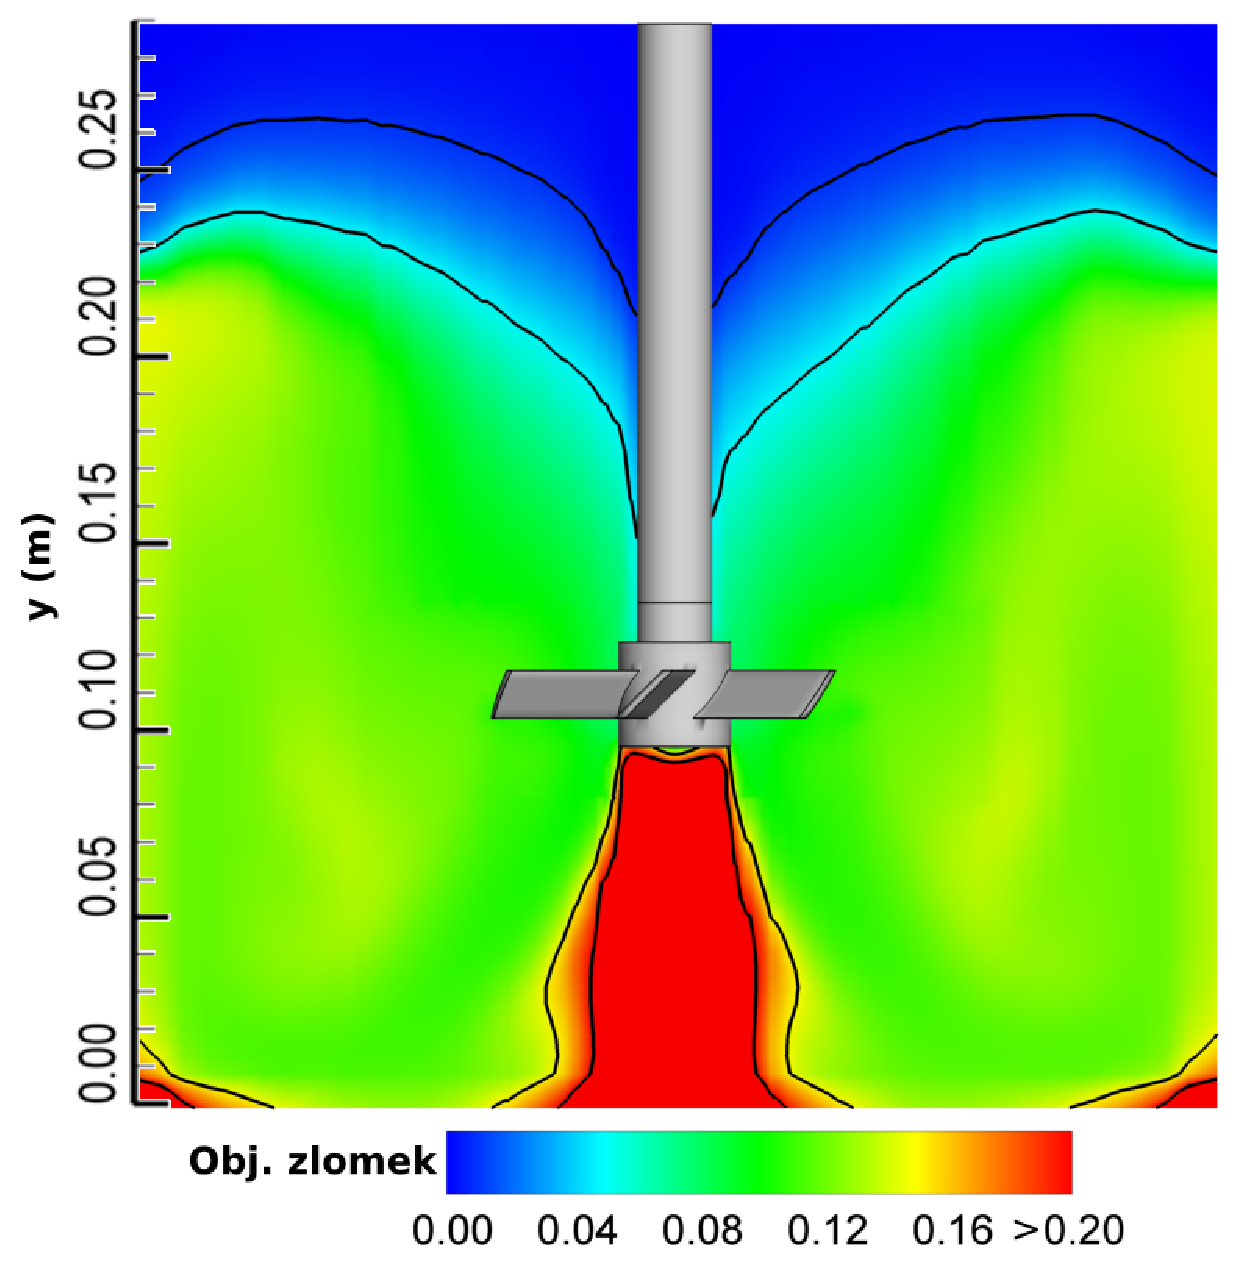
\includegraphics[scale=0.36]{Results/CloudHeight/w10-4s.eps}} 
  \qquad 
  \subfloat[experiment]{\label{fig:h-w10-4s-exp}\includegraphics[scale=0.35]{Results/CloudHeight/pvp7-vol10-4s.eps}}
  \caption{Vznos pevné fáze $\kula{N=\SI{4}{\per\second}}$}
  \label{fig:h-w10-4s}
\end{figure}

Vlivem nárůstu rychlosti otáčení míchadla na \SI{5}{\per\second} došlo ke zvýšení výšky suspezního mraku zhruba na \SI{27}{\centi\meter} (viz. obr. \ref{fig:h-w10-5s-exp}). Zmíněný jev byl taktéž pozorován pomocí CFD simulace, což ilustruje řez nádobou \ref{fig:h-w10-5s-num}. Stanovená výška vznosu pevné fáze v tomto případě činila \SI{28.3}{\centi\meter}. 
\newpage

\begin{figure}[t!]
 \centering
  \subfloat[simulace]{\label{fig:h-w10-5s-num}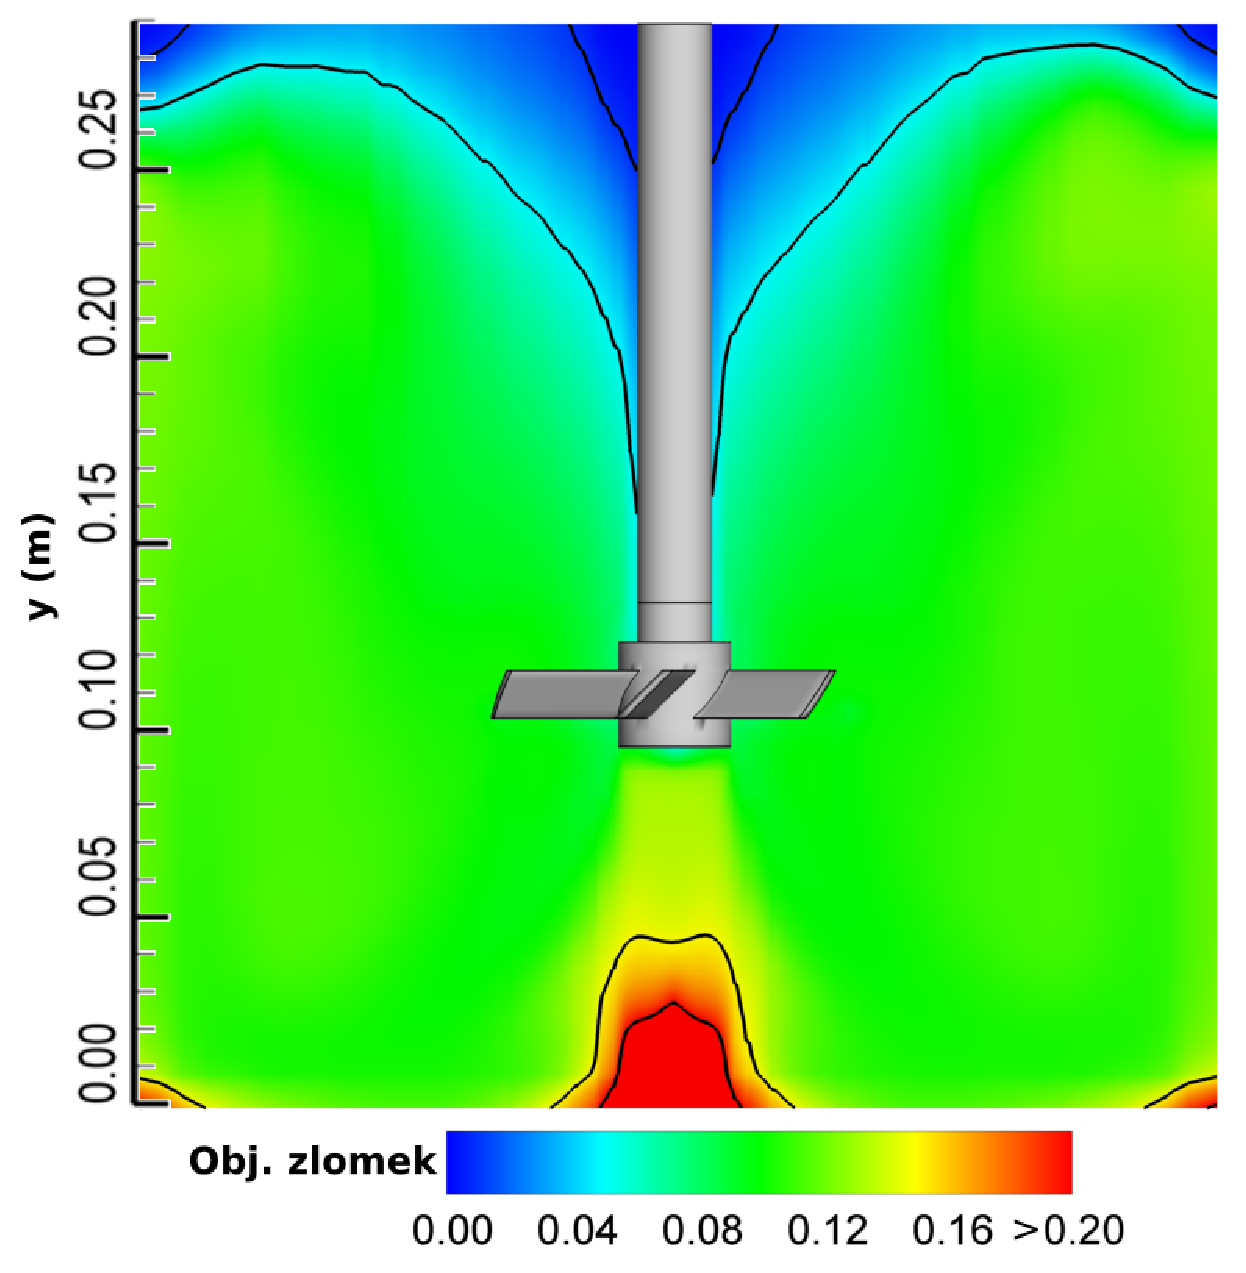
\includegraphics[scale=0.36]{Results/CloudHeight/w10-5s.eps}} 
  \qquad 
  \subfloat[experiment]{\label{fig:h-w10-5s-exp}\includegraphics[scale=0.34]{Results/CloudHeight/pvp7-vol10-5s.eps}}
  \caption{Vznos pevné fáze $\kula{N=\SI{5}{\per\second}}$}
  \label{fig:h-w10-5s}
\end{figure}
Poslední skupina obrázků \ref{fig:h-w10-6s} zachycuje stav suspenze při frekvenci otáčení míchadla \SI{6}{\per\second}. Z obrázku \ref{fig:h-w10-6s-exp} lze vidět, že pevná fáze je praticky rozptýlena v celé nádrži, a proto výška suspezního mraku je téměř totožná s výškou plnění nádoby. Obdobný závěr vyplynul i z výsledků ziskaných pomocí CFD simulace (obr. \ref{fig:h-w10-6s-num}), jenž stanovila výšku tohoto mraku na \SI{28.5}{\centi\meter}.

\begin{figure}[h!]
 \centering
  \subfloat[simulace]{\label{fig:h-w10-6s-num}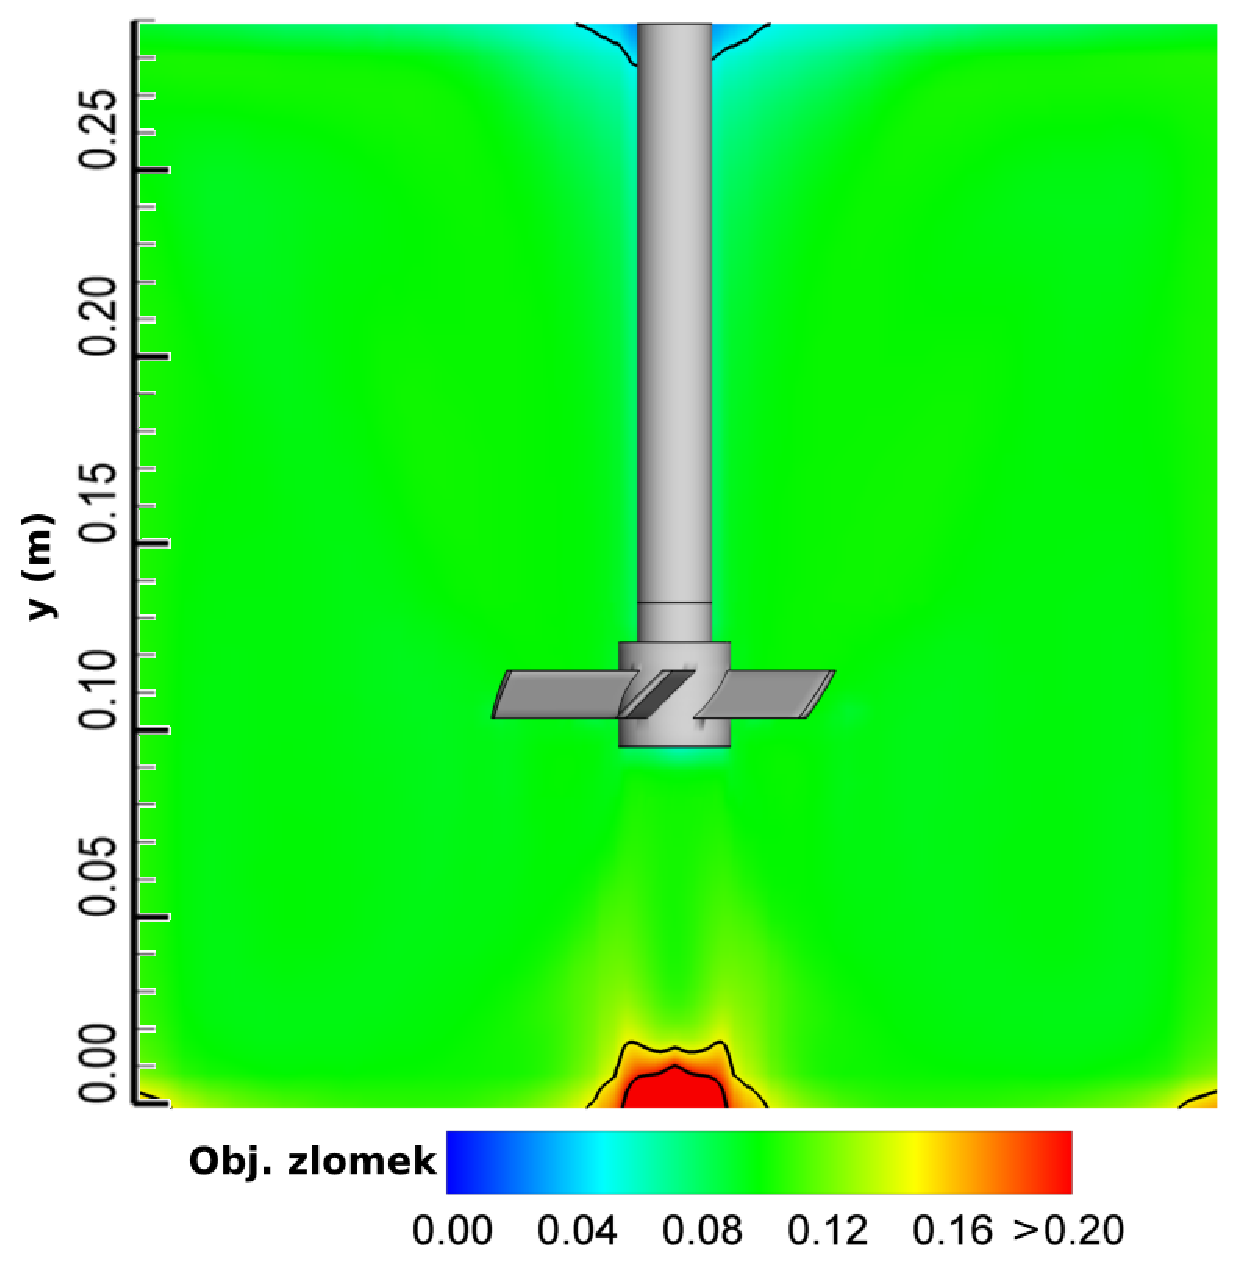
\includegraphics[scale=0.36]{Results/CloudHeight/w10-6s.eps}} 
  \qquad 
  \subfloat[experiment]{\label{fig:h-w10-6s-exp}\includegraphics[scale=0.305]{Results/CloudHeight/pvp7-vol10-6s.eps}}
  \caption{Vznos pevné fáze $\kula{N=\SI{6}{\per\second}}$}
  \label{fig:h-w10-6s}
\end{figure}
\newpage

V průběhu nestacionární CFD simulace byla kromě výšky vznosu pevné určována kvalita suspenze ($\sigma$ -- vztah \ref{eq:kvasus}). Získané výsledky pro jednotlivé frekvence otáčení míchadla jsou uvedeny v grafu \ref{grf:qa}. Pro lepší přehlednost jsou tyto závislosti zobrazeny po jedné sekundě simulace. Dle očekávání se čas potřebný k dosažení stavu úplné suspendace s rostoucí rychlostí rotace míchadla zkracoval. V případě $N=\SI{4}{\per\second}$ tato doba přibližně činila \SI{5.7}{\second}, kdežto při $N=\SI{6}{\per\second}$ se zkrátila více než dvojnásobně na zhruba \SI{2.5}{\second}. Navíc v čase kolem \SI{6}{\second} byl zaznamenán přechod do stavu homogenní suspendace pro nejvýše zvolenou frekvenci otáčení míchadla. 

\begin{grf}[h!]
 \centering
  \includegraphics[scale=0.45]{Results/CloudHeight/qa.eps}
  \caption{Průběh kvality suspenze}
  \label{grf:qa}
\end{grf}

\subsection{Srovnání modelů Eulerian-Eulerian a Eulerian-Granular}

\section{Doba homogenizace}
Doba homogenizace v daných systémech byla vyhodnocena pomocí techniky CFD s využitím dříve napočítaných rychlostních polí. Během vlastního stanovení byla řešena pouze transportní rovnice stopovací látky, což znatelně snížilo výpočetní náročnost celého procesu. V průběhu simulací byly zaznamenávány okamžité hodnoty koncentrací stopovací látky v závislosti na čase. Z uložených dat byla poté doba homogenizace určena jako čas potřebný k ustálení této koncentrace v rozmezí \SI{\pm 5}{\percent} její rovnovážné hodnoty.

Nasimulovaný průběh homogenizace indikační látky v řezu nádobou je znázorněn na obrázcích \ref{fig:t}. Jednalo se o systém tvořený vodou a pevnou fází o koncentraci \volproc{5}, přičemž frekvence otáčení míchadla činila \SI{6}{\per\second}. Na obr. \ref{fig:t0} je dobře vidět místo, kde došlo k nadávkování stopovací látky.

\begin{figure}[h!]
 \centering

  \subfloat[$t=\SI{0}{\second}$]{\label{fig:t0}\includegraphics[scale=0.38]{Results/MixingTime/voda-6s/t0.eps}}  
  \qquad             
  \subfloat[{$t=\SI{2}{\second}$}]{\label{fig:t2}\includegraphics[scale=0.38]{Results/MixingTime/voda-6s/t2.eps}}
  \\
  \subfloat[{$t=\SI{5}{\second}$}]{\label{fig:t5}\includegraphics[scale=0.38]{Results/MixingTime/voda-6s/t5.eps}}
  \qquad
  \subfloat[{$t=\SI{7}{\second}$}]{\label{fig:t7}\includegraphics[scale=0.38]{Results/MixingTime/voda-6s/t7.eps}}
  \caption{Koncentrace stopovací látky pro systém voda--PVC \volproc{5} $\kula{N=\SI{6}{\per\second}}$}
  \label{fig:t}
\end{figure}

Následují grafické závislosti bezrozměrné koncentrace stopovací látky na době homogenizace stanovené pomocí techniky CFD. Pro srovnání jsou v grafech vyneseny černou barvou experimentální údaje, které pomocí vodivostní metody stanovila \citet{pav11}. Pro snížení potřebného výpočetního času byly především zkoumány případy s vyšší hodnotou rychlosti rotace míchadla. 

Grafy \ref{fig:homvoda} zachycují výše zmíněné závislosti pro dvoufázový systém reprezentovaný vodou a kuličkami z PVC o koncentraci 5, 10 a \volproc{15} při frekvenci otáčení míchadla \SI{6}{\per\second}. Z vyobrazených průběhů je patrná dobrá shoda mezi experimentálním měřením a výsledky simulací.

\begin{grf}[h!]
 \centering
  \subfloat[\volproc{5} PVC]{\label{fig:homvoda-w5}\includegraphics[scale=0.43]{Results/MixingTime/voda-6s/5/grafy.eps}} 
  \\ 
  \subfloat[\volproc{10} PVC]{\label{fig:homvoda-w10}\includegraphics[scale=0.43]{Results/MixingTime/voda-6s/10/grafy.eps}}
\end{grf}
\newpage

\begin{grf}[t!]
  \addtocounter{subgrf}{2}
  \centering
  \subfloat[\volproc{15} PVC]{\label{fig:homvoda-w15}\includegraphics[scale=0.45]{Results/MixingTime/voda-6s/15/grafy.eps}} 
  \caption{Homogenizační křivka pro vodnou suspenzi $\kula{N=\SI{6}{\per\second}}$}
  \label{fig:homvoda}
\end{grf}
\noindent Kromě vodné vsádky byl také simulačně určen průběh bezrozměrné koncentrace indikační látky v čase pro kapalinu \pvpP{} obsahující \volproc{5} pevné fáze. Frekvence otáčení míchadla v tomto případě činila \SI{7}{\per\second}. Získaná závislost je uvedena v grafu \ref{grf:hompvp5}.
\begin{grf}[h!]
 \centering 
  \includegraphics[scale=0.45]{Results/MixingTime/PVP5-7s/5/grafy.eps}
  \caption{Homogenizační křivka pro suspenzi \pvpP{} a \volproc{5} PVC $\kula{N=\SI{7}{\per\second}}$}
  \label{grf:hompvp5}
\end{grf}
\newpage

Všechny

\begin{table}[h!]
\centering
\caption{Určené vlastnosti kapalné a pevné fáze}
\label{tab:mixtime}
\begin{tabular}{llrc}
\toprule
\textbf{Fáze} & \textbf{Veličina} & \textbf{Hodnota} &\textbf{Jednotka} \\
\midrule

voda \\
	& hustota & \num{999.50} & \si{\kilogram\per\cubic\meter} \\
	& dynamická viskozita & \num{1.138} & \si{\milli\pascal\second} \\
\pvpP \\
	& hustota & \num{1011.44} & \si{\kilogram\per\cubic\meter} \\
	& dynamická viskozita & \num{5.050} & \si{\milli\pascal\second} \\
\pvpS \\
	& hustota & \num{1024.18} & \si{\kilogram\per\cubic\meter} \\
	& dynamická viskozita & \num{7.615} & \si{\milli\pascal\second} \\
PVC \\
	& hustota & \num{1136.0} & \si{\kilogram\per\cubic\meter} \\
	& průměr & \num{1.02} & \si{\milli\meter} \\
	& mezerovitost & \num{0.384} & -- \\

\bottomrule
\end{tabular}
\end{table}
	\chapter*{Seznam symbolů}
\addcontentsline{toc}{chapter}{Seznam symbolů}

\renewcommand\arraystretch{1.5}
\begin{tabularx}{\textwidth}{@{}p{1.0cm} X r@{}}
	$b$ & šířka narážky & \si{\meter} \\
	$c$ & koncentrace & \si{\mole\per\cubic\meter} \\
	$c^{*}$ & bezrozměrná koncentrace & --\\
	$C$ & vzdálenost míchadla ode dna nádoby & \si{\meter} \\
	$C_{D0}$ & odporový koeficient podle Schillera-Naumanna & -- \\ 
	$C_{D}$ & odporový koeficient &  -- \\
	$d_{s}$ & průměr částice & \si{\meter} \\
	$D$ & průměr míchadla & \si{\meter} \\
	
	$\vec{f}_{ext}$ & objemová síla působící na objemový element & \si{\newton\per\cubic\meter} \\
	$\vec{f}_{int}$ & povrchová síla působící na objemový element & \si{\newton\per\cubic\meter} \\
	$\vec{F}_{ad}$ & další síly & \si{\newton} \\
	$\vec{F}_{D}$ & odporová síla & \si{\newton} \\
	$\vec{F}_{g}$ & gravitační síla & \si{\newton} \\
	$\vec{F}_{vz}$ & vztlaková síla & \si{\newton} \\
	$\vec{g}$ & gravitační zrychlení & \si{\meter\per\second\squared} \\
	$H$ & výška plnění nádoby & \si{\meter} \\
	$K$ & koeficient mezifázového sdílení hybnosti & \si{\kilogram\per\cubic\meter\per\second} \\
	$m_{p}$ & hmotnost částice & \si{\kilogram} \\
	
	$p$ & tlak & \si{\pascal} \\
	$\vec{R}$ & mezifázová odporová síla působící na objemový element & \si{\newton\per\cubic\meter} \\
	$Re_{p}$ & Reynoldsovo kritérium pro pevnou částici &  --\\
	$t$ & čas & \si{\second} \\
	$T$ & vnitřní průměr nádoby & \si{\meter} \\
	$U$ & napětí & \si{\volt} \\
	$\vec{v}_{p}$ & rychlost & \si{\meter\per\second} \\
\end{tabularx}


\subsubsection*{Řecké symboly}
\begin{tabularx}{\textwidth}{@{}p{1.0cm} X r@{}}
$\alpha$ & objemový zlomek& --\\
$\eta$ & dynamická viskozita & \si{\pascal\second} \\
$\lambda$ & Kolmogorovo mikroměřítko  & \si{\meter} \\
$\rho$ & hustota & \si{\kilogram\per\cubic\meter} \\
$\bar{\tau}$ & deviátor tenzoru napětí& \si{\pascal} \\
\end{tabularx}

\subsubsection*{Spodní indexy}
\begin{tabularx}{\textwidth}{@{}p{1.0cm} X r@{}}
$f$ & tekutina & \\
$i$ & $i$-tá fáze & \\
$j$ & $j$-tá fáze & \\
$p$ & pevná částice & \\
$s$ & pevná fáze & \\
\end{tabularx}


\subsubsection*{Zkratky}
\begin{tabularx}{\textwidth}{@{}p{1.0cm} X }
CFD & computational fluid dynamics  \\
PVC & polyvinylchlorid  \\
PVP & polyvinylpyrrolidon  \\
UDF & user defined function  \\
\end{tabularx}

	\normalsize{}
	%\setlength{\bibhang}{0pt} odsazen prvního řádku bibliografie
	\begin{thebibliography}{99}
\addcontentsline{toc}{chapter}{Bibliography}

\bibitem[Armenante \textit{et al.}, 1998]{arm98} Armenante, P. M., Nagamine, E. U., Susanto, J., 1998. Determination of correlations to predict the minimum agitation speed for complete solid suspension in agitated vessels. \textit{Can J Chem Eng}, \textbf{76}, 413--419

\bibitem[Baldi \textit{et al.}, 1978]{bal78} Baldi, G., Conti, R., Alaria, E., 1978. Complete suspension of particles in mechanically agitated vessels. \textit{Chem Eng Sci}, \textbf{33}, 21--25 

\bibitem[Brucato \textit{et al.}, 1998]{bru98} Brucato, A., Grisafi, F., Montante, G., 1998. Particle drag coefficients in turbulent fluids. \textit{Chem Eng Sci}, \textbf{43}, 3, 3295--3314

\bibitem[Derksen, 2003]{derk03} Derksen, J.J., 2003. Numerical Simulation of solid suspension in a stirredtank. \textit{AIChE J}, \textbf{49}, 11, 2700--2714

\bibitem[Ihme \textit{et al.}, 1972]{ihme72} Ihme, F., Schmidt-Traub H., Brauer, H., 1972. Theoretische untersuchung \"uber die Umstr\"omung und den Stoff\"ubergang an Kugeln. \textit{Chem.-Ing.-Tech.}, \textbf{44}, 306

\bibitem[Ishii-Zuber, 1979]{ish79} Ishii, M., Zuber, N., 1979, Drag coefficient and relative velocity in bubbly, droplet or particulate flows, \textit{AIChE J}, \textbf{28}, 843--855 

\bibitem[Kresta and Wood, 1991]{kre91} Kresta, S. M., Wood, P. E., 1991. Prediction of three-dimensional turbulent flow in stirred tanks. \textit{AIChE J}, \textbf{37}, 448--460 

\bibitem[Ljungqvist and Rasmuson, 2001]{lju01} Ljungqvist, M., Rasmuson, A., 2001. Numerical simulation of the two-phase flow in an axially stirred reactor. \textit{Trans AIChE}, \textbf{79}, Part A, 533--546

\bibitem[Micheletti \textit{et al.}, 2003]{miche03} Micheletti, L., Nikiforaki, L., Lee, K.C., Yianeeskis, M., 2003. Integral and Local Concentration Characteristics of Moderate to Dense Solid-Liquid Suspensions. \textit{11$^{th}$ European Conference on Mixing}, Bamberg, Germany


\bibitem[e.g.\ Nienow, 1968]{nie68} Nienow, A. W., 1968. Suspension of solid particles in turbine agitated baffled vessels. \textit{Chem Eng Sci}, \textbf{23}, 1453--1459 

\bibitem[Oshinowo and Bakker, 2001]{oshi02} Oshinowo, L. M., Bakker, A., 2002. CFD modeling of solids suspensions in stirred tanks. \textit{Symposium on Computational Modeling of Metals, Minerals and Materials}, February 17-21, Seattle, Washington 

\bibitem[Schiller-Naumann, 1935]{schi32} Schiller, L., Naumann, Z., 1935. A drag coefficient correlation. \textit{Z. Ver. Deutsch. Ing.}, \textbf{77}, 318--320

\bibitem[Syamlal and O'Brien, 1993]{syam93} Syamlal, M., O'Brien, T.J., 1993. MFIX Documentation: Theory Guide. \textit{National Technical Information Service}, \textbf{1}, Springfield, Virginia 

\bibitem[Zwietering, 1957]{zwi58} Zwietering, T. N., 1958. Suspending of solid particles in liquid by agitators. \textit{Chem Eng Sci}, \textbf{8}, 244--253 

\end{thebibliography}

	\chapter*{Příloha}
\label{sec:priloha}
\addcontentsline{toc}{chapter}{Příloha}
Zde jsou uvedeny vytvořené zdrojové kódy uživatelsky definovaných funkcí pro dané modely koeficientu odporu. Online repositář je možné nalézt na adrese:\\ \href{http://code.google.com/p/mixing-udfs/source/browse/\#hg\%2FDragCoefModels}{http://code.google.com/p/mixing-udfs/source/browse/\#hg\%2FDragCoefModels}


\lstinputlisting{Models.c}

\lstinputlisting{SchillerNauman.h}

\end{document}
